% Week 9: Decoding Strategies - Complete Redesign (Template Conformant)
% 37 main slides + 25 appendix slides = 62 total
% NEW: 6 problems -> 6 solutions pedagogy + vocabulary visualization
% Enhanced: November 13, 2025 | Template: template_beamer_final.tex

\documentclass[8pt,aspectratio=169]{beamer}
\usetheme{Madrid}
\usepackage{graphicx}
\usepackage{booktabs}
\usepackage{adjustbox}
\usepackage{multicol}
\usepackage{amsmath}
\usepackage{tikz}

% Math commands
\DeclareMathOperator*{\argmax}{argmax}
\DeclareMathOperator*{\argmin}{argmin}
\DeclareMathOperator{\softmax}{softmax}

% Color definitions (complete palette from template)
\definecolor{mlblue}{RGB}{0,102,204}
\definecolor{mlpurple}{RGB}{51,51,178}
\definecolor{mllavender}{RGB}{173,173,224}
\definecolor{mllavender2}{RGB}{193,193,232}
\definecolor{mllavender3}{RGB}{204,204,235}
\definecolor{mllavender4}{RGB}{214,214,239}
\definecolor{mlorange}{RGB}{255,127,14}
\definecolor{mlgreen}{RGB}{44,160,44}
\definecolor{mlred}{RGB}{214,39,40}
\definecolor{mlgray}{RGB}{127,127,127}

% Additional colors for template compatibility
\definecolor{lightgray}{RGB}{240,240,240}
\definecolor{midgray}{RGB}{180,180,180}

% Apply custom colors to Madrid theme
\setbeamercolor{palette primary}{bg=mllavender3,fg=mlpurple}
\setbeamercolor{palette secondary}{bg=mllavender2,fg=mlpurple}
\setbeamercolor{palette tertiary}{bg=mllavender,fg=white}
\setbeamercolor{palette quaternary}{bg=mlpurple,fg=white}

\setbeamercolor{structure}{fg=mlpurple}
\setbeamercolor{section in toc}{fg=mlpurple}
\setbeamercolor{subsection in toc}{fg=mlblue}
\setbeamercolor{title}{fg=mlpurple}
\setbeamercolor{frametitle}{fg=mlpurple,bg=mllavender3}
\setbeamercolor{block title}{bg=mllavender2,fg=mlpurple}
\setbeamercolor{block body}{bg=mllavender4,fg=black}

% Remove navigation symbols
\setbeamertemplate{navigation symbols}{}

% Clean itemize/enumerate
\setbeamertemplate{itemize items}[circle]
\setbeamertemplate{enumerate items}[default]

% Reduce margins for more content space
\setbeamersize{text margin left=5mm,text margin right=5mm}

% Command for bottom annotation (Madrid-style)
\newcommand{\bottomnote}[1]{%
\vfill
\vspace{-2mm}
\textcolor{mllavender2}{\rule{\textwidth}{0.4pt}}
\vspace{1mm}
\footnotesize
\textbf{#1}
}

\title{Decoding Strategies}
\subtitle{Week 9 - From Probabilities to Text}
\date{November 13, 2025}

\begin{document}

% ============================================
% MAIN PRESENTATION (37 SLIDES)
% ============================================

% === SLIDE 1: TITLE (TEMPLATE LAYOUT 1) ===
\begin{frame}[plain]
\vspace{2cm}
\begin{center}
{\Huge\textbf{Decoding Strategies}}\\[0.5cm]
{\Large Week 9: From Probabilities to Text}\\[2cm]
{\normalsize November 2025}
\end{center}
\end{frame}

% === SLIDE 2: NEW - THE DECODING CHALLENGE ===
\begin{frame}[t]{The Decoding Challenge: Choosing From 50,000 Words}
\vspace{-0.3cm}
\begin{center}
\includegraphics[width=0.80\textwidth]{../figures/vocabulary_probability_bsc.pdf}
\end{center}

\vspace{3mm}
\textbf{The Question}: Given these probabilities for ``The cat \_\_'', which word should we pick?

\bottomnote{At each step, model outputs probability distribution over entire vocabulary - how do we choose?}
\end{frame}

% === SLIDE 3: CONTEXT - HOW WE GOT HERE ===
\begin{frame}[t]{Context: How We Got Here}
\vspace{-0.3cm}
\begin{center}
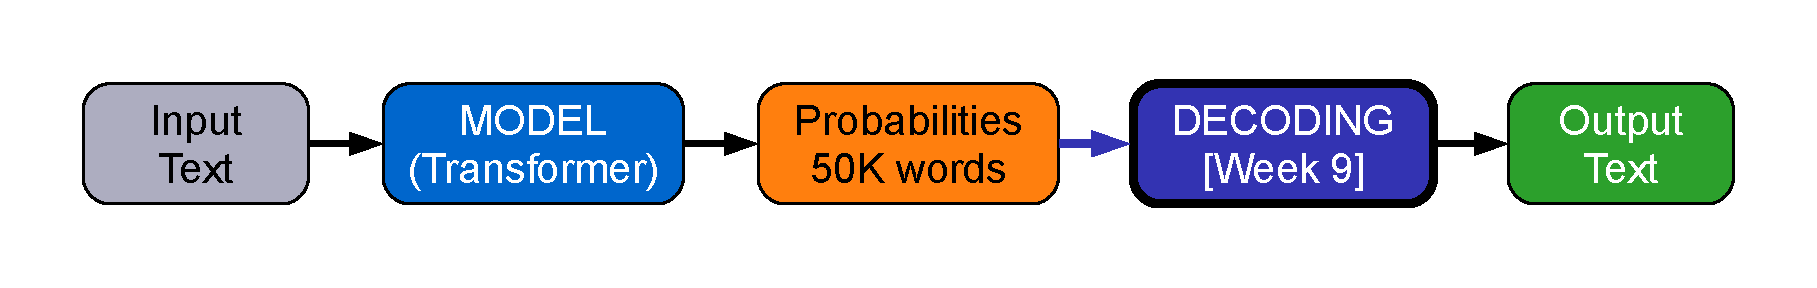
\includegraphics[width=0.75\textwidth]{../figures/prediction_to_text_pipeline_bsc.pdf}
\end{center}

\vspace{3mm}
\small
\textbf{Our Journey}:
\begin{enumerate}
\item We trained models (Weeks 3-7: RNN $\rightarrow$ Transformers $\rightarrow$ BERT/GPT)
\item They learned to predict: $P(\text{word} | \text{context})$
\item They output probability distributions over 50,000+ words
\item \textbf{Today}: How do we convert these probabilities into actual text?
\end{enumerate}

\bottomnote{Models predict probabilities. Decoding converts probabilities to text.}
\end{frame}

% === SLIDE 4: QUALITY-DIVERSITY TRADEOFF (FIXED) ===
\begin{frame}[t]{The Quality-Diversity Tradeoff}
\vspace{-0.3cm}
\begin{center}
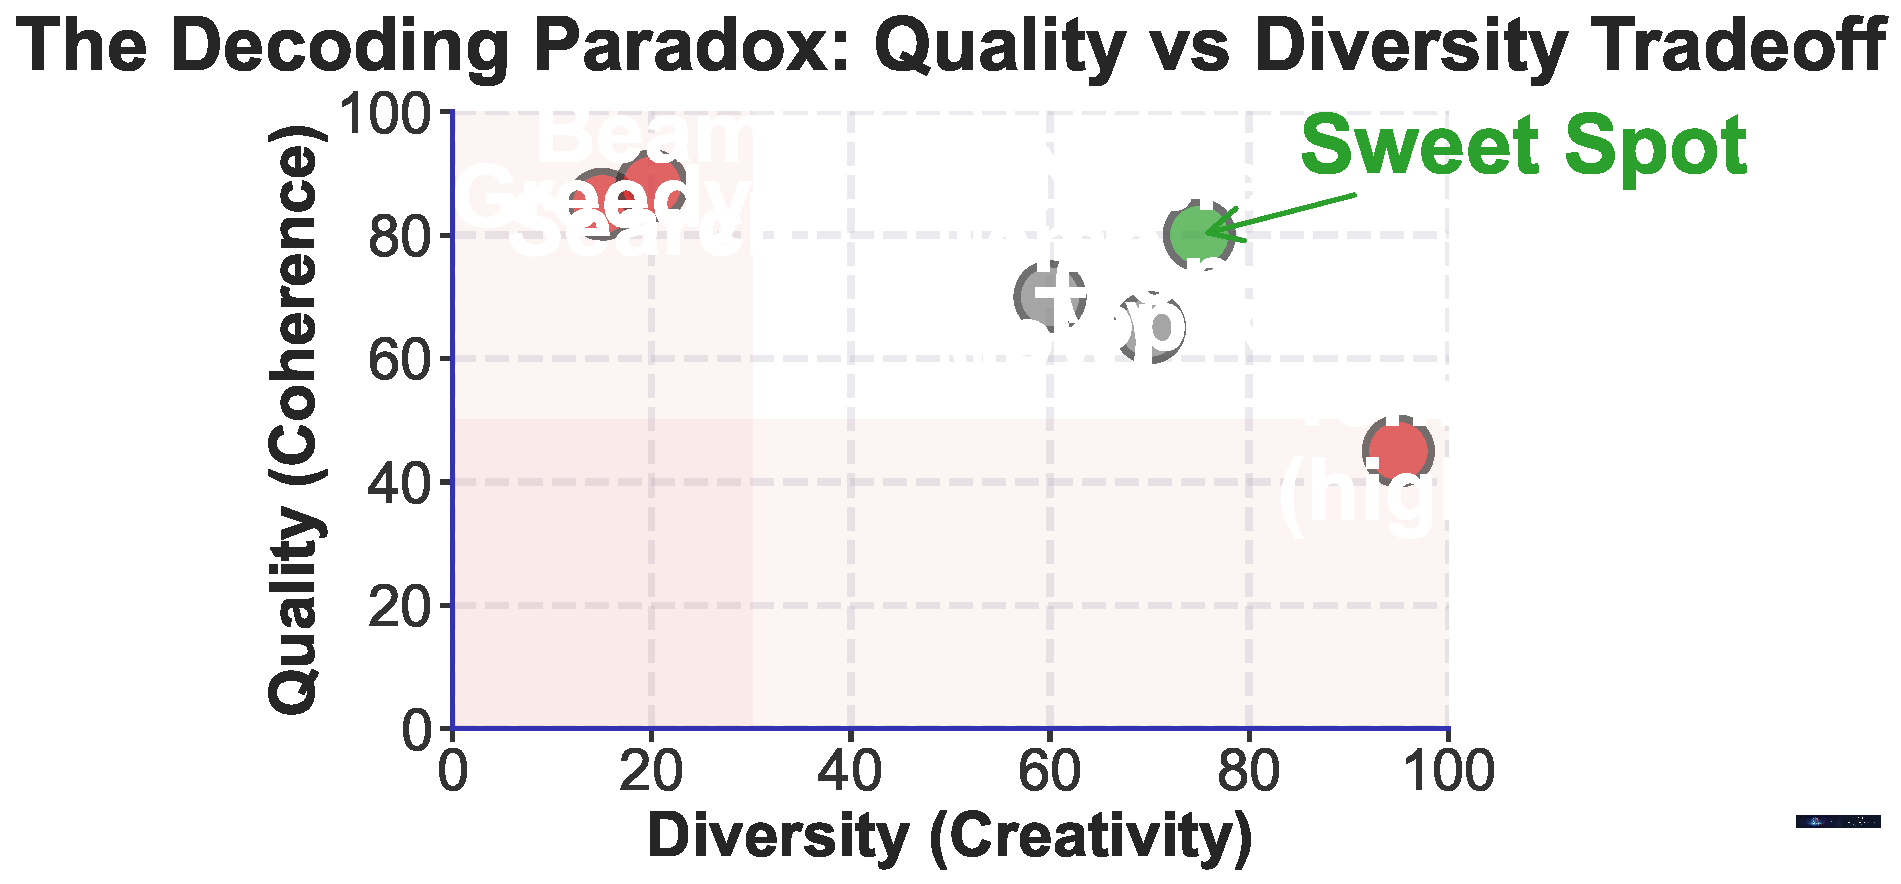
\includegraphics[width=0.70\textwidth]{../figures/quality_diversity_tradeoff_bsc.pdf}
\end{center}
\begin{center}
\textbf{Discovery Question}: Why is best text boring and creative text nonsense?
\end{center}
\bottomnote{The central challenge: How to balance coherence with creativity}
\end{frame}

% ============================================
% THE 6 PROBLEMS (Slides 5-10)
% ============================================

\begin{frame}[t]{Problem 1: Stuck in Repetition Loops}
\vspace{-0.5cm}
\begin{center}
\includegraphics[width=0.75\textwidth]{../figures/problem1_repetition_output_bsc.pdf}
\end{center}
\bottomnote{Problem 1 of 6: Greedy decoding creates loops}
\end{frame}

\begin{frame}[t]{Problem 2: No Diversity in Outputs}
\vspace{-0.5cm}
\begin{center}
\includegraphics[width=0.75\textwidth]{../figures/problem2_diversity_output_bsc.pdf}
\end{center}
\bottomnote{Problem 2 of 6: Deterministic methods lack variation}
\end{frame}

\begin{frame}[t]{Problem 3: Too Boring or Too Crazy}
\vspace{-0.5cm}
\begin{center}
\includegraphics[width=0.75\textwidth]{../figures/problem3_balance_output_bsc.pdf}
\end{center}
\bottomnote{Problem 3 of 6: Need controlled randomness}
\end{frame}

\begin{frame}[t]{Problem 4: Missing Better Paths}
\vspace{-0.5cm}
\begin{center}
\includegraphics[width=0.75\textwidth]{../figures/problem4_paths_output_bsc.pdf}
\end{center}
\bottomnote{Problem 4 of 6: Local optimum $\neq$ global best}
\end{frame}

\begin{frame}[t]{Problem 5: Wrong Probability Distribution}
\vspace{-0.5cm}
\begin{center}
\includegraphics[width=0.75\textwidth]{../figures/problem5_distribution_output_bsc.pdf}
\end{center}
\bottomnote{Problem 5 of 6: Tail of distribution contains junk}
\end{frame}

\begin{frame}[t]{Problem 6: Speed vs Quality Tradeoff}
\vspace{-0.5cm}
\begin{center}
\includegraphics[width=0.75\textwidth]{../figures/problem6_speed_output_bsc.pdf}
\end{center}
\bottomnote{Problem 6 of 6: Better quality costs computational resources}
\end{frame}

% ============================================
% CHECKPOINT QUIZ 1
% ============================================

\begin{frame}[t]{Checkpoint Quiz 1: Match the Problem}
\begin{columns}[T]
\column{0.45\textwidth}
\textbf{Problems:}
\begin{enumerate}
\item Repetition loops
\item No diversity
\item Too boring/crazy
\item Missing better paths
\item Wrong distribution
\item Speed vs quality
\end{enumerate}

\column{0.55\textwidth}
\textbf{Match to Examples:}

\begin{itemize}
\item[\textbf{A.}] "The the the the..."
\item[\textbf{B.}] Always outputs "Yes."
\item[\textbf{C.}] Temperature too high: gibberish
\item[\textbf{D.}] Greedy misses "cat sat" for "cat walked"
\item[\textbf{E.}] Low-prob words get sampled
\item[\textbf{F.}] Need to process 50K words each step
\end{itemize}
\end{columns}

\vspace{5mm}
\pause
\begin{center}
\colorbox{mlgreen!30}{\parbox{0.85\textwidth}{
\centering
\textbf{Answers:} 1→A, 2→B, 3→C, 4→D, 5→E, 6→F\\[2mm]
\textit{Understanding problems is key to choosing solutions!}
}}
\end{center}

\bottomnote{Quiz 1: Can you identify each decoding problem?}
\end{frame}

% ============================================
% THE 6 SOLUTIONS (Slides 11-16)
% ============================================

\begin{frame}[t]{Solution 1 $\rightarrow$ Beam Search: Explore Multiple Paths}
\begin{columns}[T]
\column{0.48\textwidth}
\textbf{Problem 1 Recap}:

Greedy decoding: Trapped in loops

Always picks highest probability

Misses better sequences

\vspace{3mm}
{\color{red}\textbf{Need}}: Way to explore alternatives

\column{0.48\textwidth}
\textbf{Solution: Beam Search}:

Keep top-k paths at each step

Explore k=3-5 hypotheses simultaneously

Pick best complete sequence at end

\vspace{3mm}
{\color{blue}\textbf{Result}}: Finds better sequences than greedy
\end{columns}

\vspace{5mm}
\textbf{How it solves Problem 1}: Maintains multiple candidates, avoids greedy trap

\bottomnote{Solution 1 of 6: Beam search for better quality}
\end{frame}

\begin{frame}[t]{Solution 2 $\rightarrow$ Temperature: Add Controlled Randomness}
\begin{columns}[T]
\column{0.48\textwidth}
\textbf{Problem 2 Recap}:

No diversity: Same output always

Deterministic selection

No creativity

\vspace{3mm}
{\color{red}\textbf{Need}}: Controlled randomness

\column{0.48\textwidth}
\textbf{Solution: Temperature}:

Reshape probability distribution

T < 1: More focused

T > 1: More random

Sample from adjusted distribution

\vspace{3mm}
{\color{blue}\textbf{Result}}: Different outputs each time
\end{columns}

\vspace{5mm}
\textbf{How it solves Problem 2}: Sampling introduces stochasticity, enables diversity

\bottomnote{Solution 2 of 6: Temperature for creativity control}
\end{frame}

\begin{frame}[t]{Solution 3 $\rightarrow$ Top-k: Filter Unlikely Words}
\begin{columns}[T]
\column{0.48\textwidth}
\textbf{Problem 3 Recap}:

Can't balance quality \& creativity

Pure sampling too random

Greedy too boring

\vspace{3mm}
{\color{red}\textbf{Need}}: Filter bad words, keep good

\column{0.48\textwidth}
\textbf{Solution: Top-k Sampling}:

Keep only top-k most likely tokens

Cut tail of distribution

Renormalize probabilities

Sample from filtered set

\vspace{3mm}
{\color{blue}\textbf{Result}}: Diverse but not nonsensical
\end{columns}

\vspace{5mm}
\textbf{How it solves Problem 3}: Fixed cutoff prevents tail sampling while allowing creativity

\bottomnote{Solution 3 of 6: Top-k for controlled sampling}
\end{frame}

\begin{frame}[t]{Solution 4 $\rightarrow$ Nucleus: Dynamic Vocabulary Cutoff}
\begin{columns}[T]
\column{0.48\textwidth}
\textbf{Problem 4 Recap}:

Top-k has fixed cutoff

Peaked distribution: Wastes probability

Flat distribution: Still allows junk

\vspace{3mm}
{\color{red}\textbf{Need}}: Adaptive cutoff

\column{0.48\textwidth}
\textbf{Solution: Nucleus (Top-p)}:

Choose smallest set with cumulative prob $\geq$ p

Adapts to distribution shape

Peaked $\rightarrow$ small nucleus (2-3 words)

Flat $\rightarrow$ large nucleus (50+ words)

\vspace{3mm}
{\color{blue}\textbf{Result}}: Automatic quality-diversity balance
\end{columns}

\vspace{5mm}
\textbf{How it solves Problem 4}: Dynamic cutoff adapts to each prediction step

\bottomnote{Solution 4 of 6: Nucleus for adaptive sampling}
\end{frame}

\begin{frame}[t]{Solution 5 $\rightarrow$ Top-k + Temperature: Hybrid Control}
\begin{columns}[T]
\column{0.48\textwidth}
\textbf{Problem 5 Recap}:

Temperature alone doesn't filter tail

Top-k alone doesn't control randomness

Need both filtering AND tuning

\vspace{3mm}
{\color{red}\textbf{Need}}: Combine strategies

\column{0.48\textwidth}
\textbf{Solution: Hybrid Methods}:

Apply temperature THEN top-k

Or: Apply nucleus THEN temperature

Leverages strengths of both

Production systems use combinations

\vspace{3mm}
{\color{blue}\textbf{Result}}: Fine-grained control over generation
\end{columns}

\vspace{5mm}
\textbf{How it solves Problem 5}: Layered strategies handle multiple issues simultaneously

\bottomnote{Solution 5 of 6: Hybrid methods for comprehensive control}
\end{frame}

\begin{frame}[t]{Solution 6 $\rightarrow$ Contrastive: Explicit Degeneration Prevention}
\begin{columns}[T]
\column{0.48\textwidth}
\textbf{Problem 6 Recap}:

Repetition even with sampling

Long generation degenerates

Context similarity causes loops

\vspace{3mm}
{\color{red}\textbf{Need}}: Explicit repetition penalty

\column{0.48\textwidth}
\textbf{Solution: Contrastive Search}:

Score = Probability - $\alpha \times$ Similarity

Penalize tokens similar to recent context

Balance quality with diversity

Modern standard for long text

\vspace{3mm}
{\color{blue}\textbf{Result}}: Human-like text without repetition
\end{columns}

\vspace{5mm}
\textbf{How it solves Problem 6}: Direct similarity penalty prevents copying context

\bottomnote{Solution 6 of 6: Contrastive for degeneration-free generation}
\end{frame}

% ============================================
% CHECKPOINT QUIZ 2
% ============================================

\begin{frame}[t]{Checkpoint Quiz 2: Which Method for Which Problem?}
\begin{columns}[T]
\column{0.5\textwidth}
\textbf{Match Solution to Problem:}

\begin{enumerate}
\item Beam Search → ?
\item Temperature → ?
\item Top-k → ?
\item Nucleus → ?
\item Hybrid → ?
\item Contrastive → ?
\end{enumerate}

\column{0.5\textwidth}
\textbf{Problems to Solve:}

\begin{itemize}
\item[\textbf{A.}] Too boring OR too crazy
\item[\textbf{B.}] Missing better paths
\item[\textbf{C.}] Wrong distribution tail
\item[\textbf{D.}] No diversity
\item[\textbf{E.}] Repetition despite diversity
\item[\textbf{F.}] Dynamic vocabulary needed
\end{itemize}
\end{columns}

\vspace{5mm}
\pause
\begin{center}
\colorbox{mllavender3}{\parbox{0.85\textwidth}{
\centering
\textbf{Answers:} 1→B, 2→D, 3→A, 4→F, 5→C, 6→E\\[2mm]
\textit{Each method targets a specific failure mode!}
}}
\end{center}

\bottomnote{Quiz 2: Understanding the method-problem mapping}
\end{frame}

% ============================================
% DETAILED METHODS (Slides 17-29)
% ============================================

% === BEAM SEARCH (2 slides) ===
% Note: beam_search_visual_bsc.pdf doesn't exist, using example directly

\begin{frame}[t]{Beam Search: Step-by-Step Example}
\vspace{-0.3cm}
\begin{center}
\includegraphics[width=0.75\textwidth]{../figures/beam_search_example_bsc.pdf}
\end{center}
\bottomnote{Worked example shows why beam search finds better sequences than greedy}
\end{frame}

\begin{frame}[t]{Beam Search: Algorithm \& Settings}
\small
\begin{columns}[T]
\column{0.48\textwidth}
\textbf{Algorithm}:

\begin{enumerate}
\item Start: Keep top-k tokens
\item Expand: Generate continuations for each
\item Score: Multiply probabilities
\item Prune: Keep top-k sequences
\item Repeat until END token
\end{enumerate}

\vspace{3mm}
\textbf{Scoring}:

$$\text{score}(y_1...y_t) = \prod_{i=1}^t P(y_i | y_{<i})$$

With length normalization:

$$\text{score} = \frac{1}{t} \sum_{i=1}^t \log P(y_i | y_{<i})$$

\column{0.48\textwidth}
\textbf{Best For}:
\begin{itemize}
\item Machine translation
\item Summarization
\item Question answering
\item Tasks with ``correct'' answer
\end{itemize}

\vspace{3mm}
\textbf{Parameters}:

Width = 3-5 (translation)

Width = 10 (diverse outputs)

\vspace{3mm}
\textbf{Tradeoffs}:

+ Better quality than greedy

+ Diverse hypotheses

- Still deterministic

- 4-5$\times$ slower than greedy

\end{columns}
\bottomnote{Beam search is the workhorse for deterministic tasks}
\end{frame}

% === TEMPERATURE (2 slides) ===
\begin{frame}[t]{Temperature Sampling: Control Randomness}
\vspace{-0.3cm}
\begin{center}
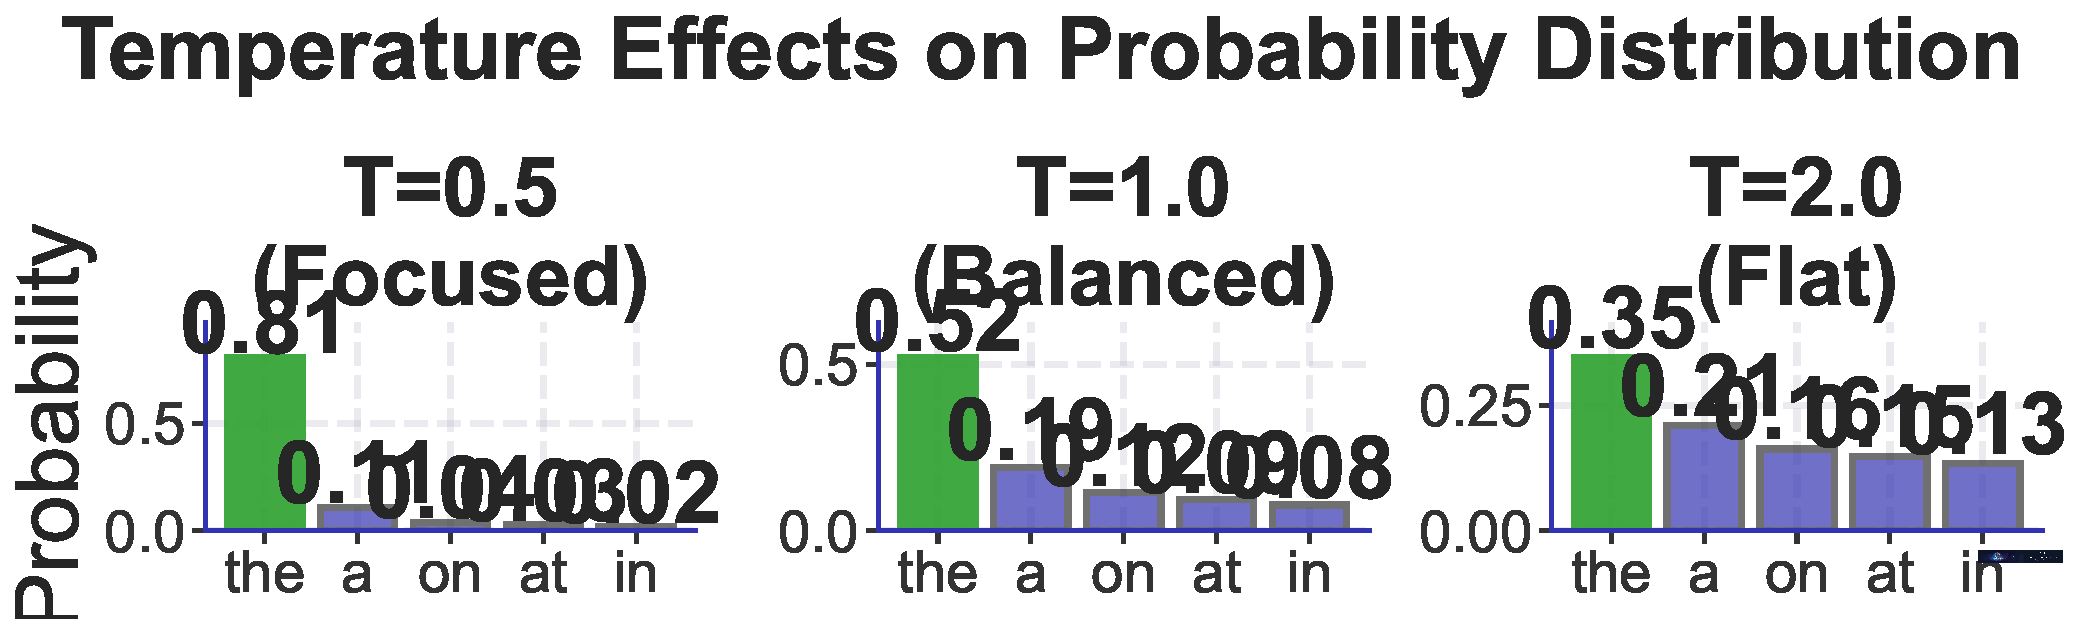
\includegraphics[width=0.65\textwidth]{../figures/temperature_effects_bsc.pdf}
\end{center}
\begin{center}
\textbf{Key Insight}: Temperature reshapes probability distribution
\end{center}
\bottomnote{T $<$ 1: more focused. T = 1: unchanged. T $>$ 1: more random}
\end{frame}

\begin{frame}[t]{Temperature: Worked Example}
\vspace{-0.3cm}
\begin{center}
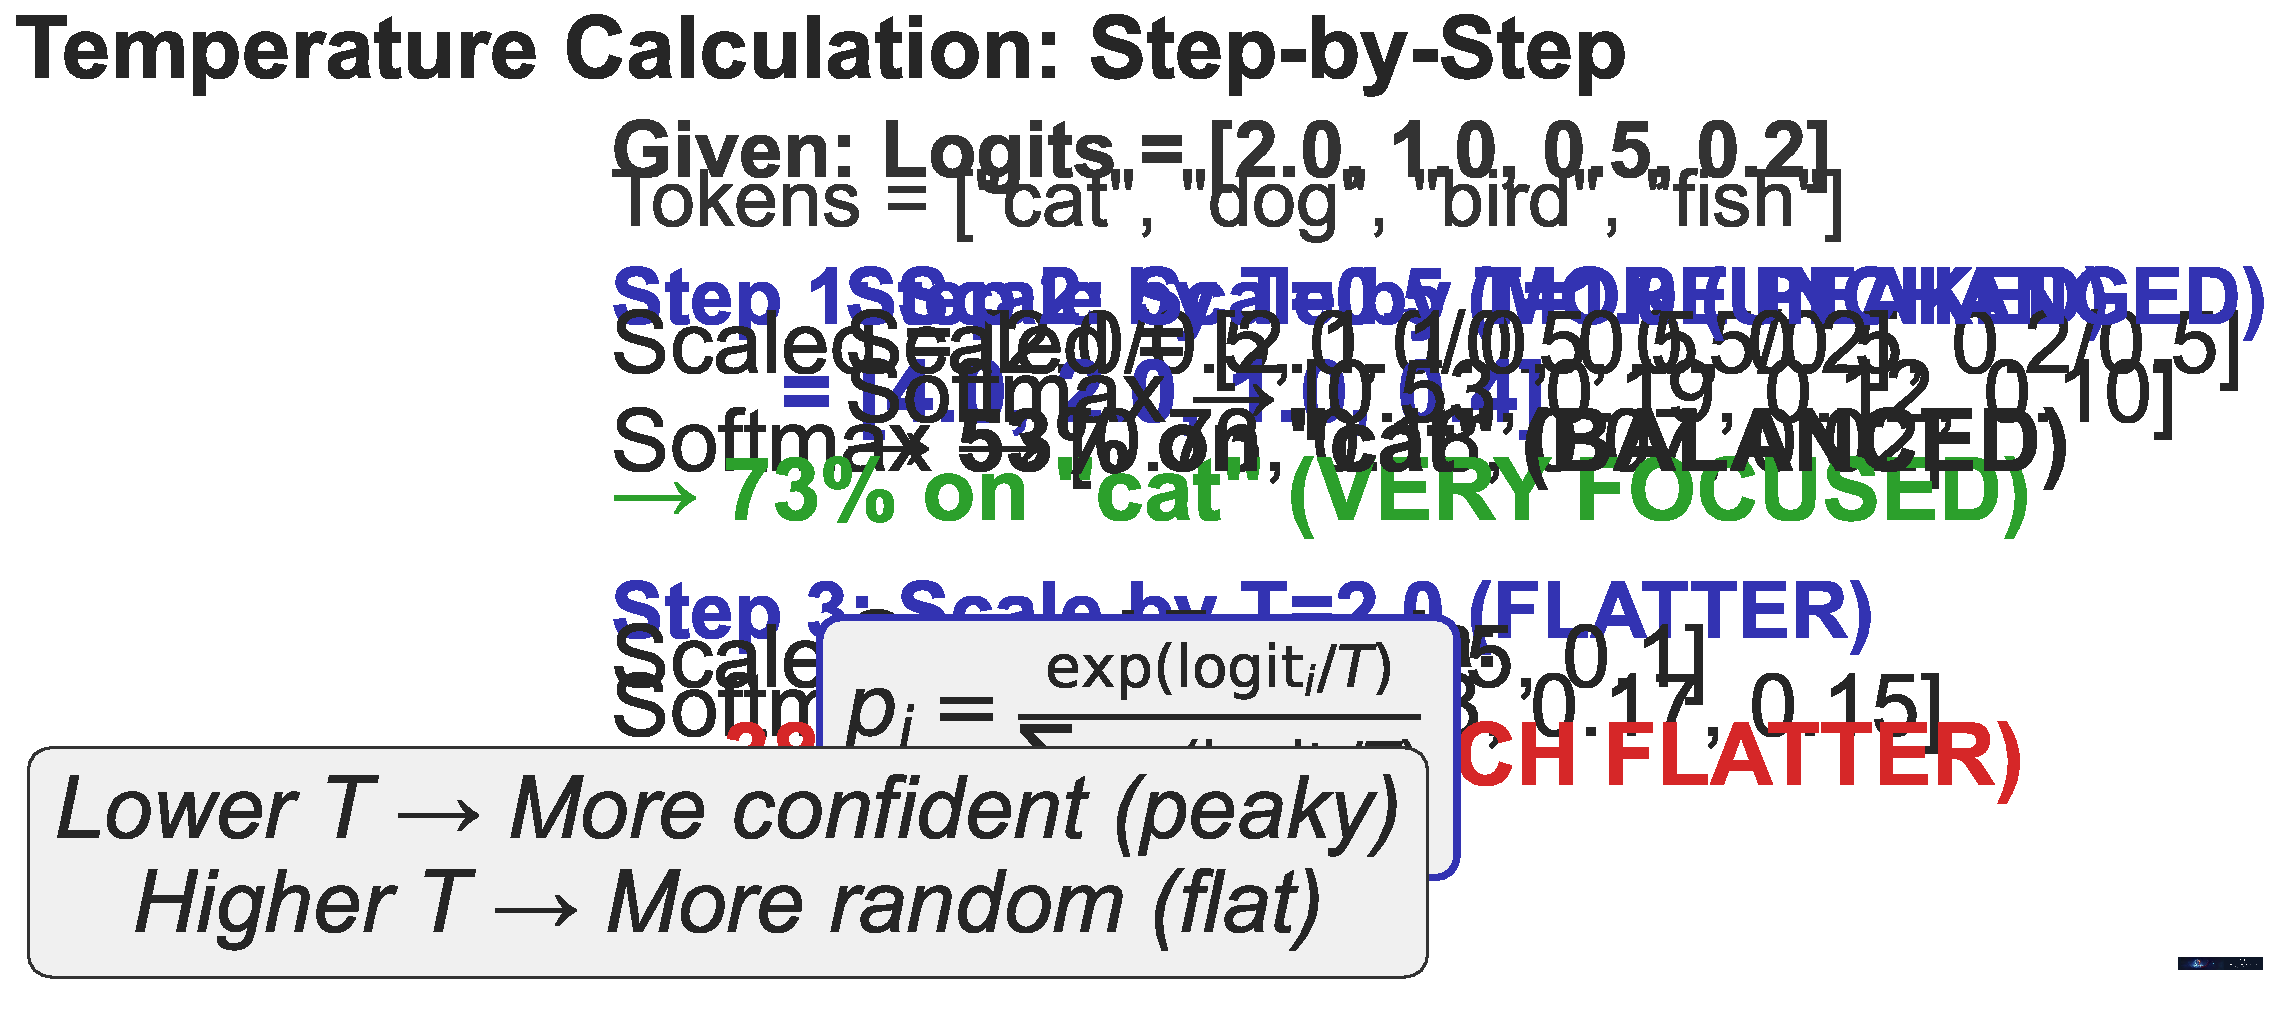
\includegraphics[width=0.70\textwidth]{../figures/temperature_calculation_bsc.pdf}
\end{center}
\bottomnote{Concrete numbers show how temperature scaling works}
\end{frame}

% === TOP-K (2 slides) ===
\begin{frame}[t]{Top-k Sampling: Filter the Tail}
\vspace{-0.3cm}
\begin{center}
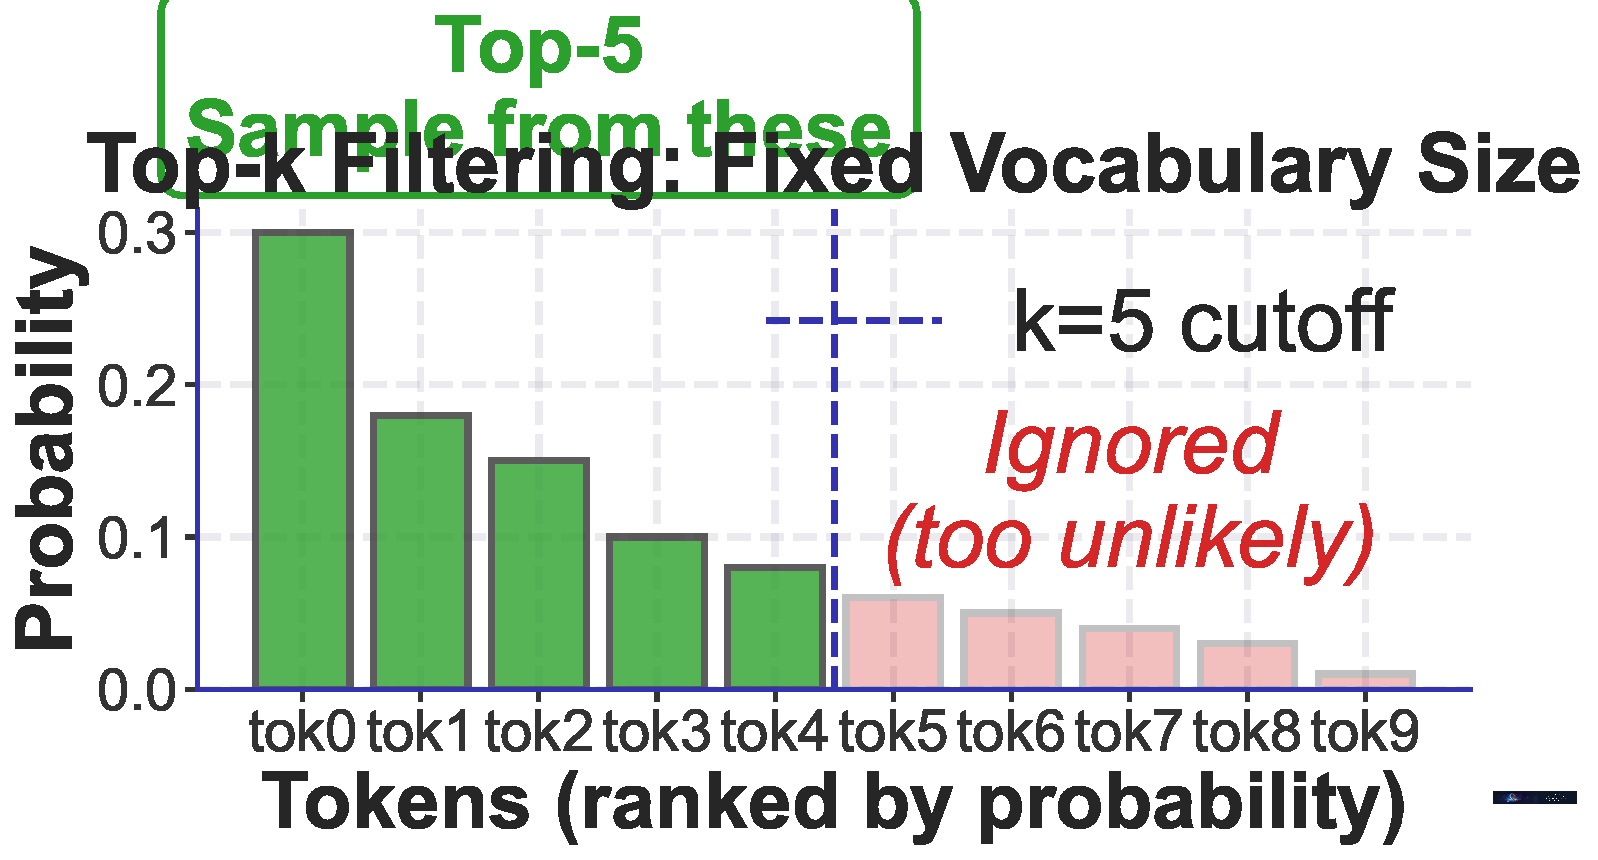
\includegraphics[width=0.70\textwidth]{../figures/topk_filtering_bsc.pdf}
\end{center}
\begin{center}
\textbf{Key Insight}: Only sample from top-k most likely tokens
\end{center}
\bottomnote{Prevents sampling from long tail of unlikely words}
\end{frame}

% Slide removed - topk_example_bsc.pdf not generated

% === NUCLEUS (2 slides) ===
\begin{frame}[t]{Nucleus (Top-p) Sampling: Dynamic Cutoff}
\vspace{-0.3cm}
\begin{center}
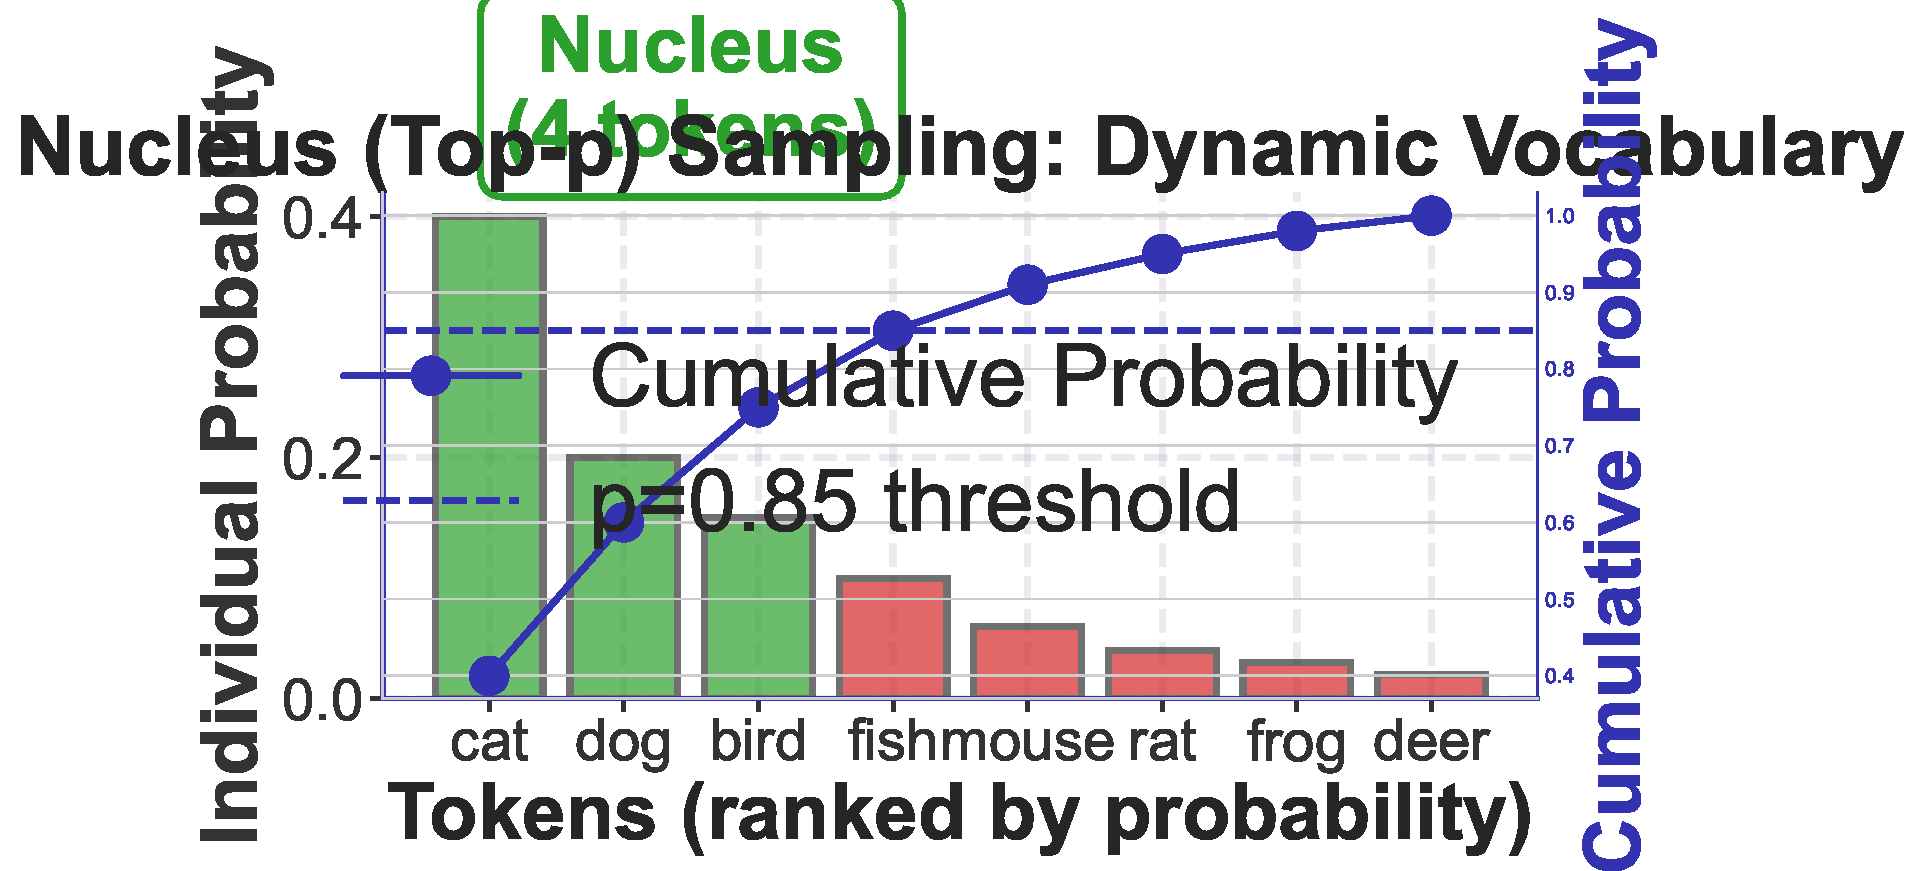
\includegraphics[width=0.70\textwidth]{../figures/nucleus_process_bsc.pdf}
\end{center}
\begin{center}
\textbf{Key Insight}: Adapt vocabulary size to distribution shape
\end{center}
\bottomnote{Nucleus size grows/shrinks based on probability spread}
\end{frame}

\begin{frame}[t]{Nucleus: How Distribution Shape Matters}
\vspace{-0.3cm}
\begin{center}
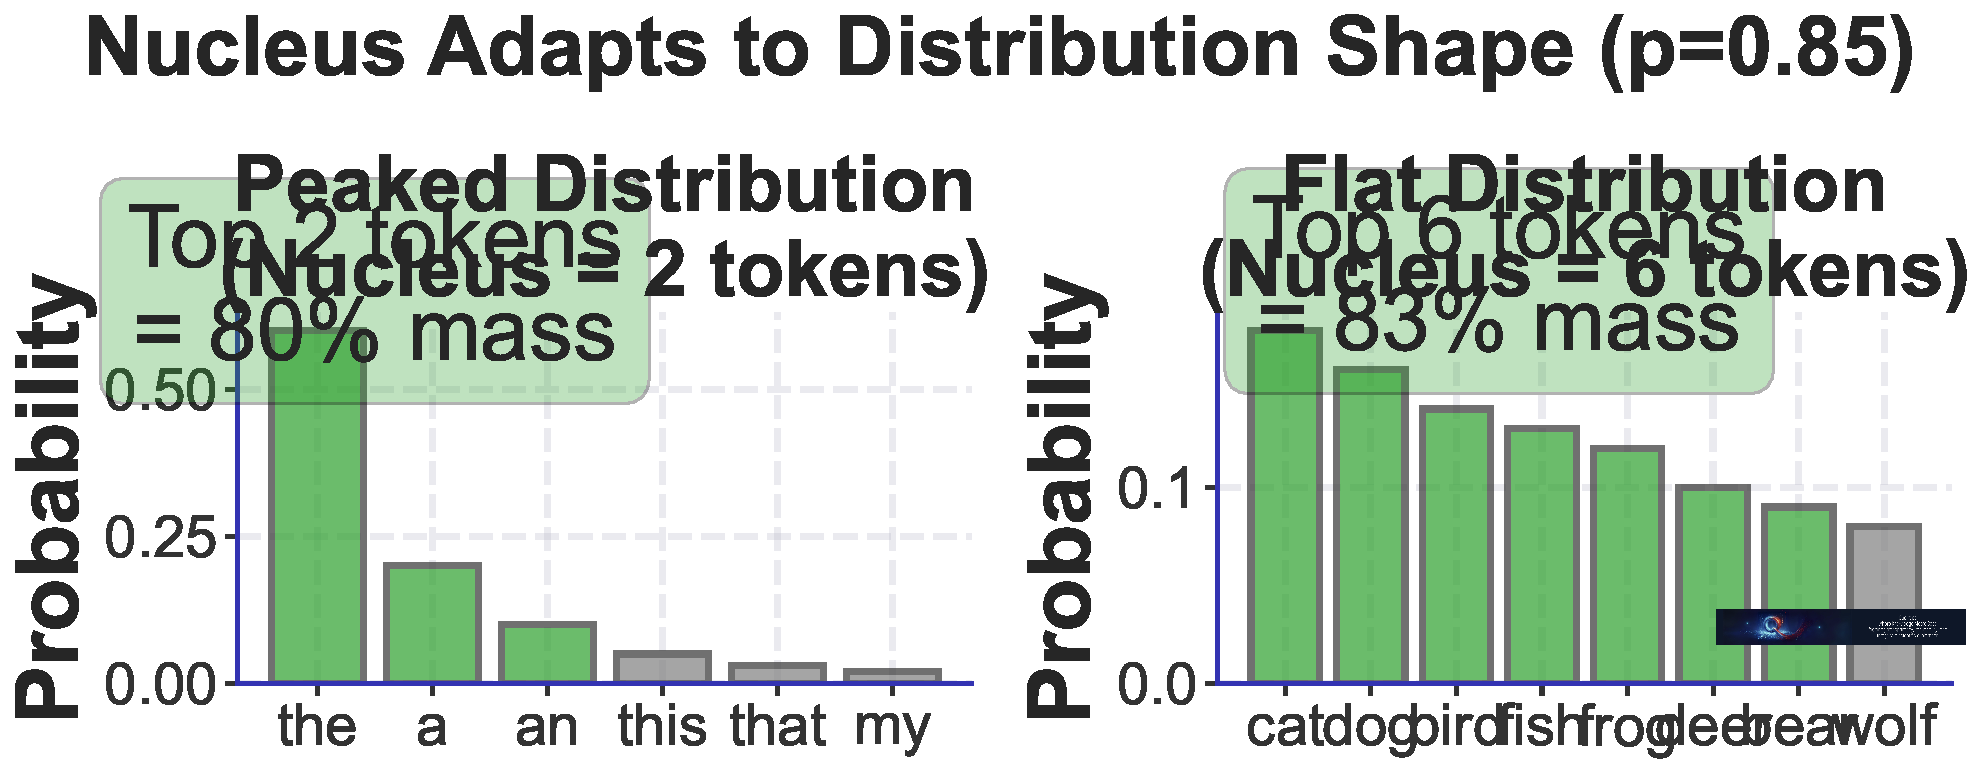
\includegraphics[width=0.70\textwidth]{../figures/nucleus_cumulative_bsc.pdf}
\end{center}
\bottomnote{Same p value gives different vocabulary sizes for peaked vs flat distributions}
\end{frame}

% === CONTRASTIVE (3 slides) ===
\begin{frame}[t]{The Degeneration Problem}
\vspace{-0.3cm}
\begin{center}
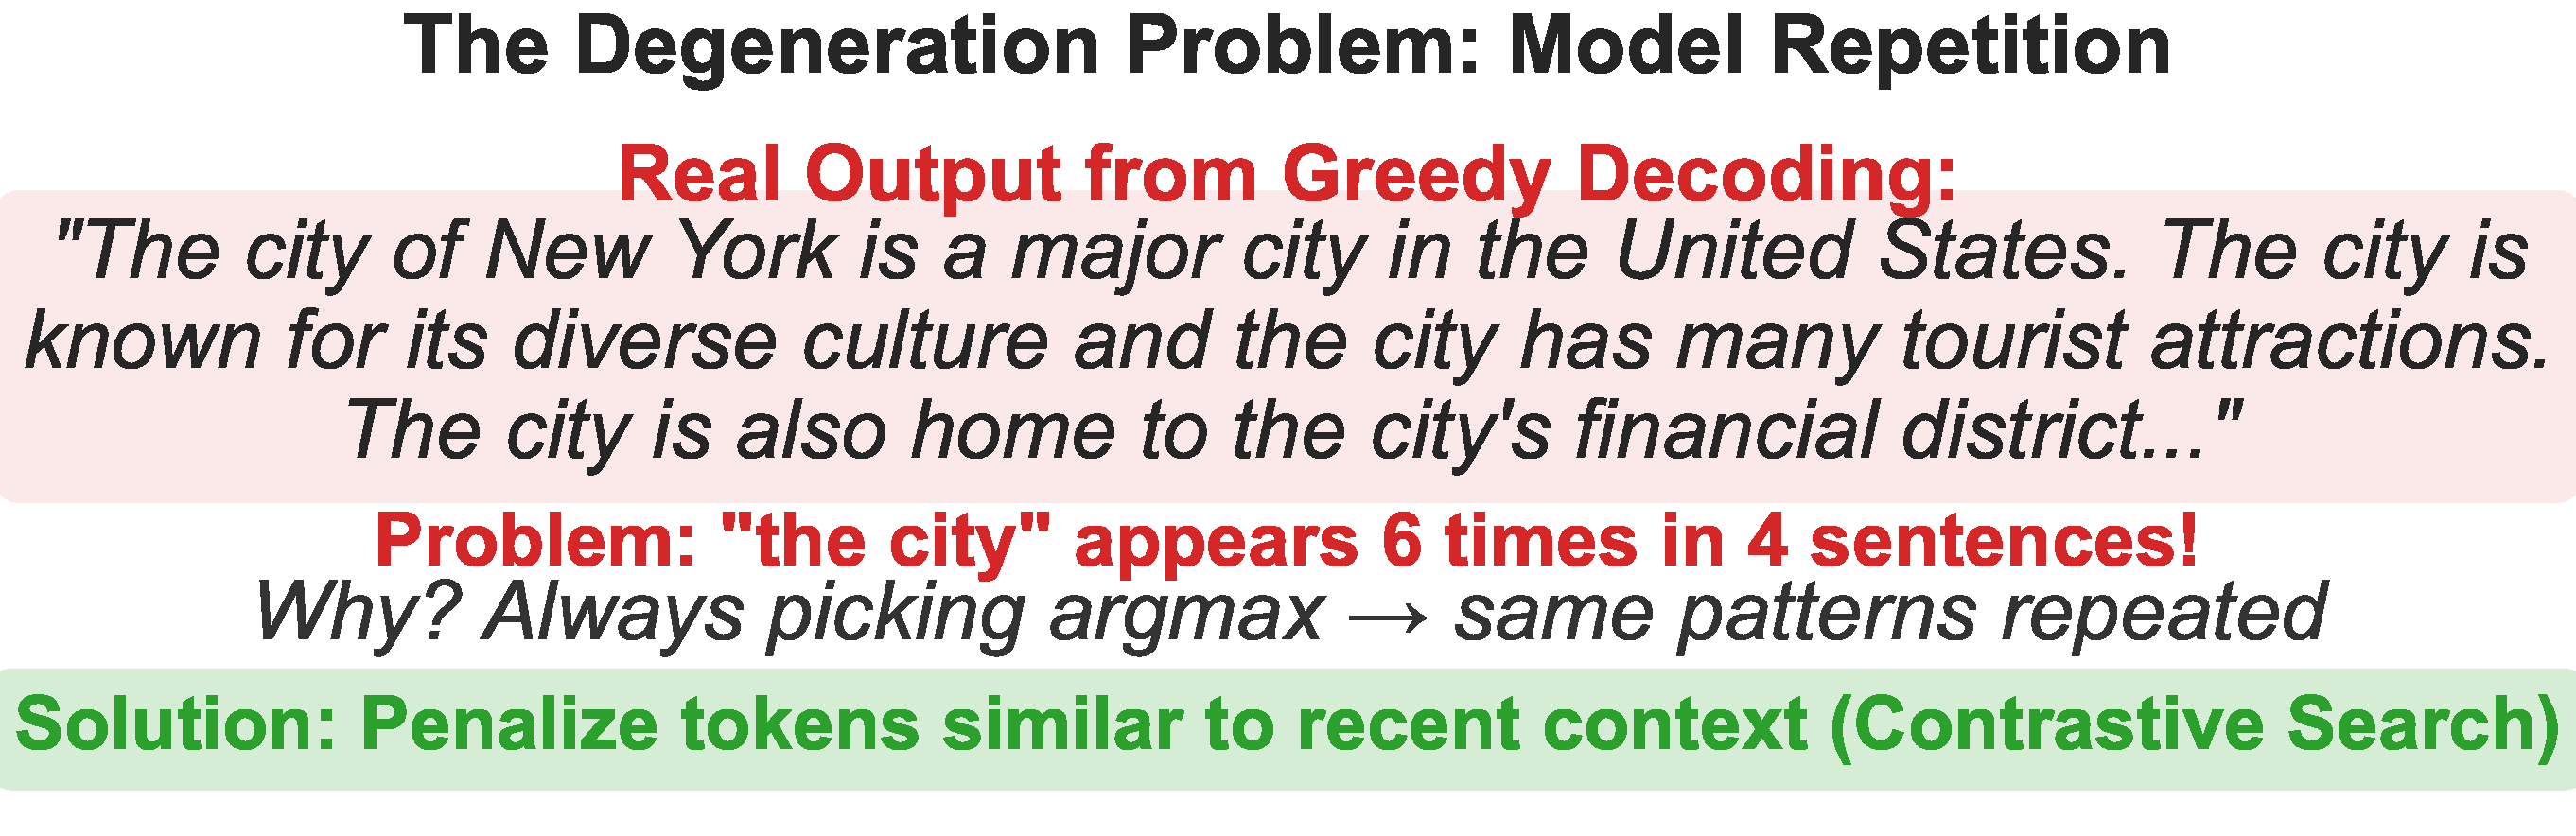
\includegraphics[width=0.70\textwidth]{../figures/degeneration_problem_bsc.pdf}
\end{center}
\begin{center}
\textbf{Discovery Question}: Why do models repeat themselves?
\end{center}
\bottomnote{Greedy and beam search maximize probability - but high probability = repeating recent context}
\end{frame}

\begin{frame}[t]{Contrastive Search: Penalize Repetition}
\vspace{-0.3cm}
\begin{center}
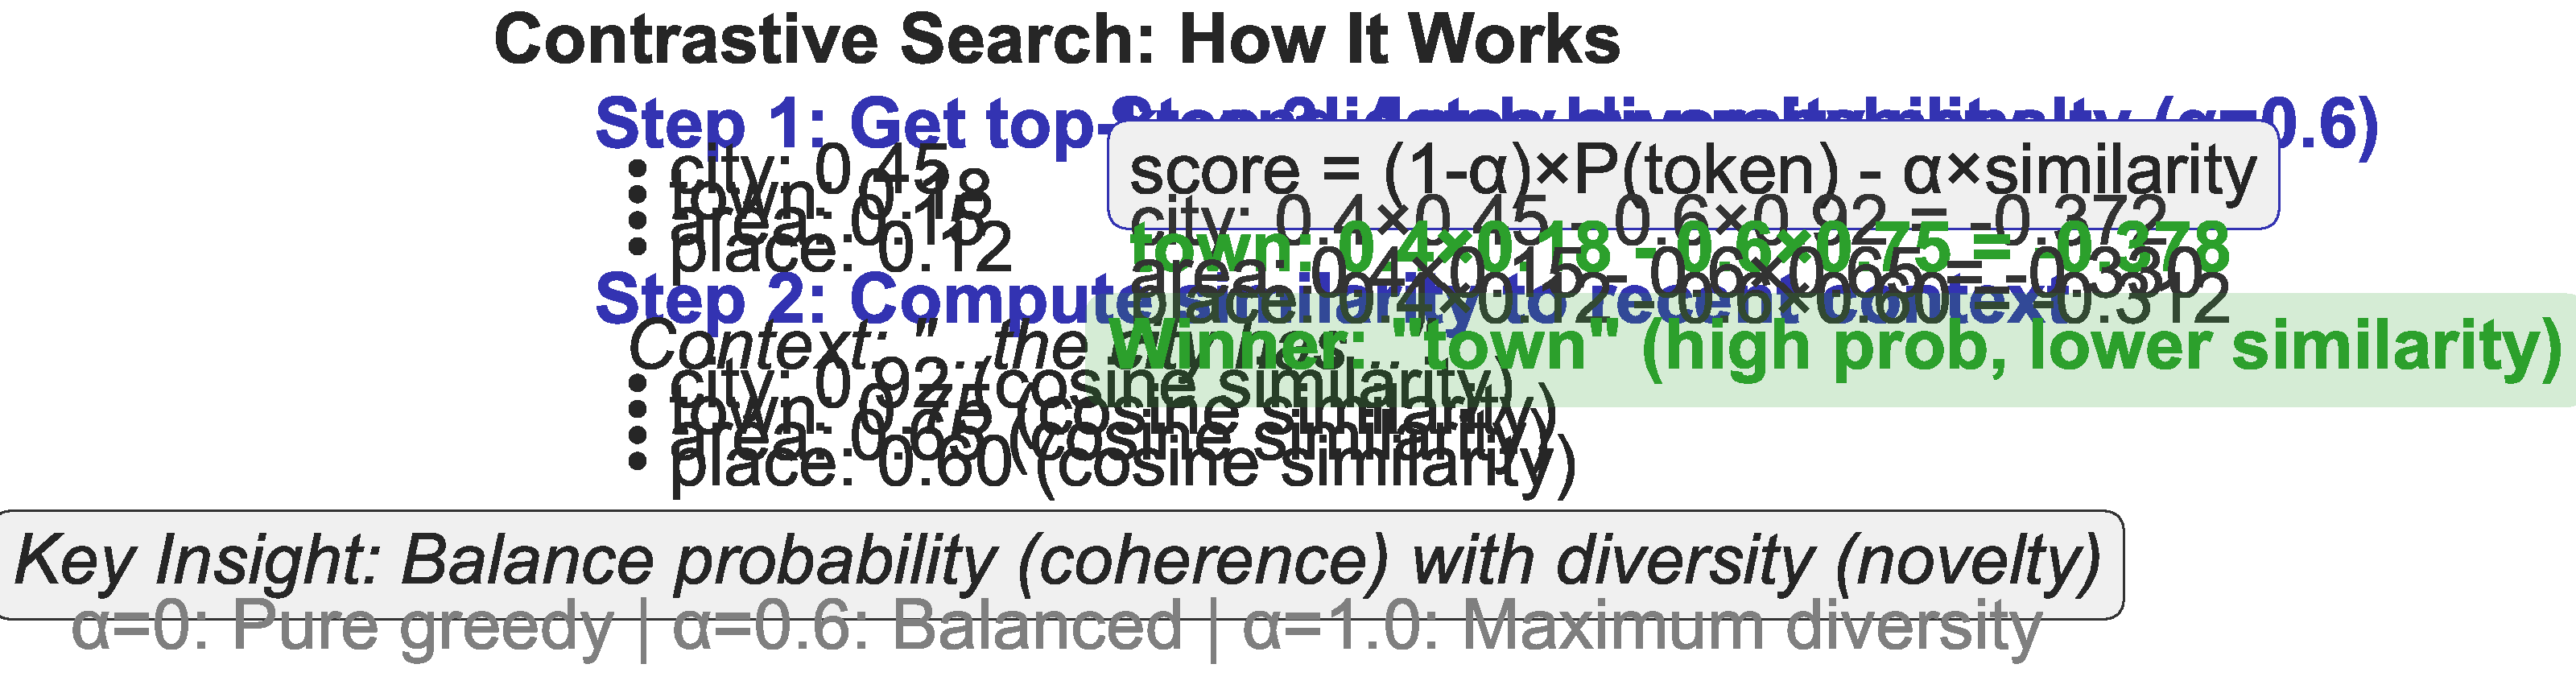
\includegraphics[width=0.70\textwidth]{../figures/contrastive_mechanism_bsc.pdf}
\end{center}
\begin{center}
\textbf{Key Insight}: Balance probability with diversity penalty
\end{center}
\bottomnote{Explicitly avoid copying recent context - prevents degeneration in long texts}
\end{frame}

% Slide removed - contrastive_vs_nucleus_bsc.pdf not generated

% === INTEGRATION (4 slides: 30-33) ===
\begin{frame}[t]{All Methods on Quality-Diversity Space}
\vspace{-0.3cm}
\begin{center}
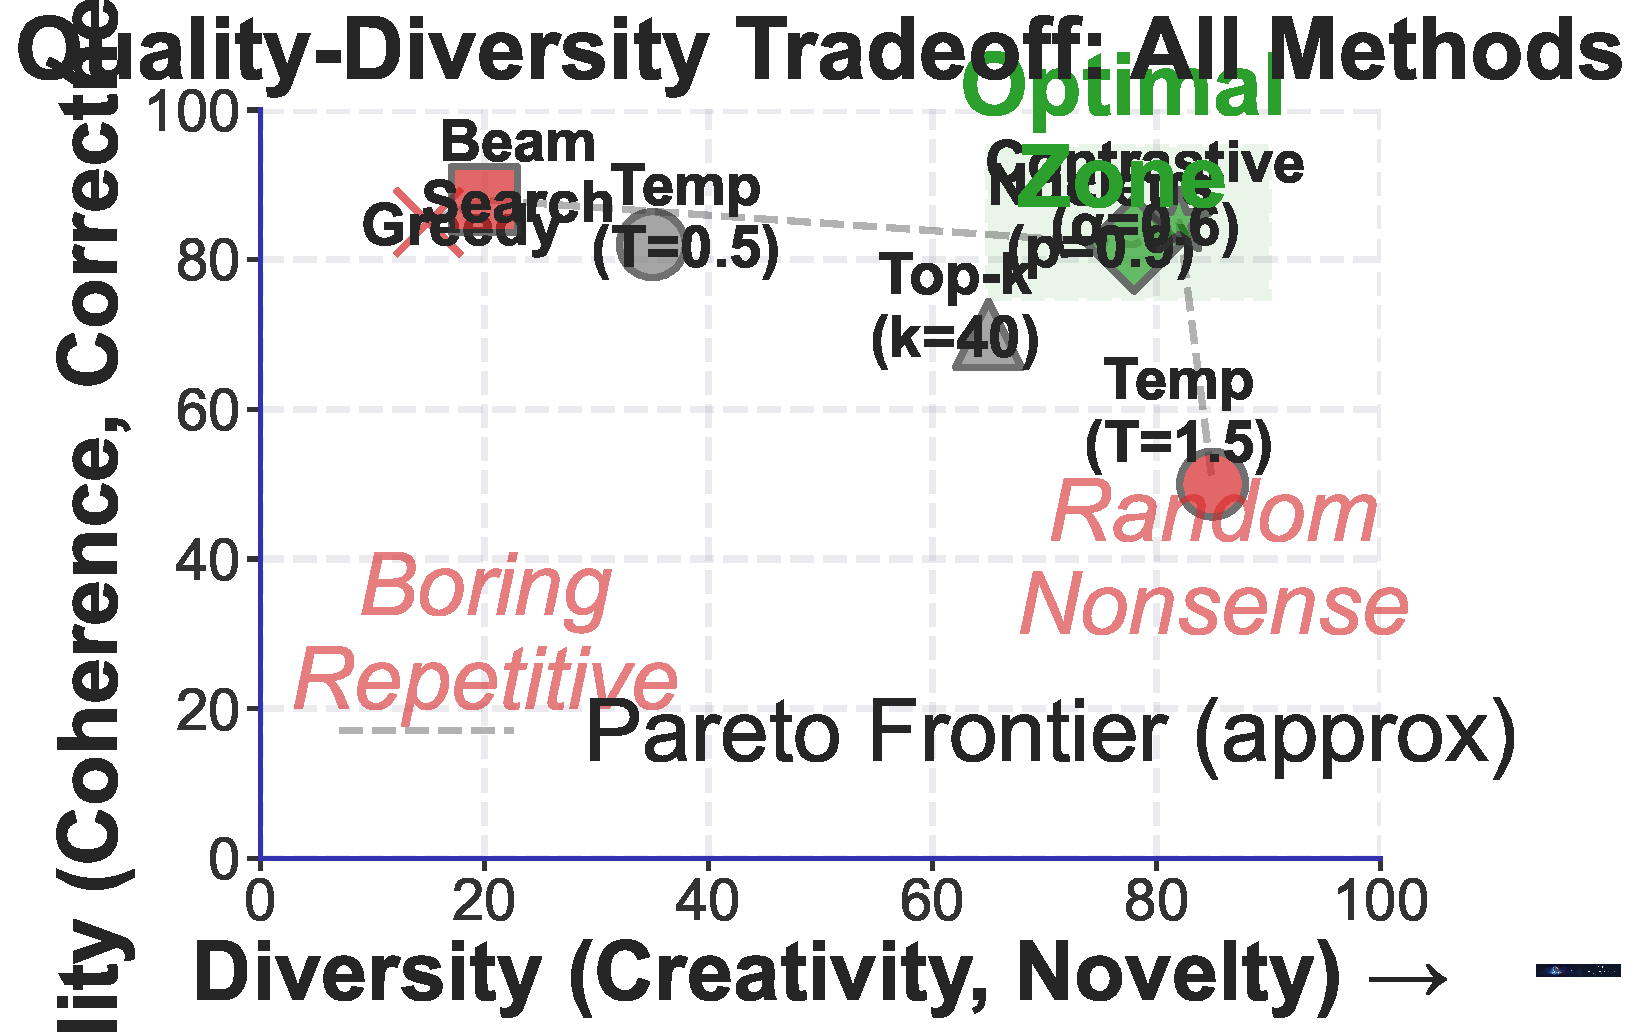
\includegraphics[width=0.70\textwidth]{../figures/quality_diversity_pareto_bsc.pdf}
\end{center}
\begin{center}
\textbf{Pareto Frontier}: No method dominates all others
\end{center}
\bottomnote{Choose based on task: deterministic tasks (left), creative tasks (right)}
\end{frame}

\begin{frame}[t]{Choosing the Right Method: Decision Tree}
\vspace{-0.3cm}
\begin{center}
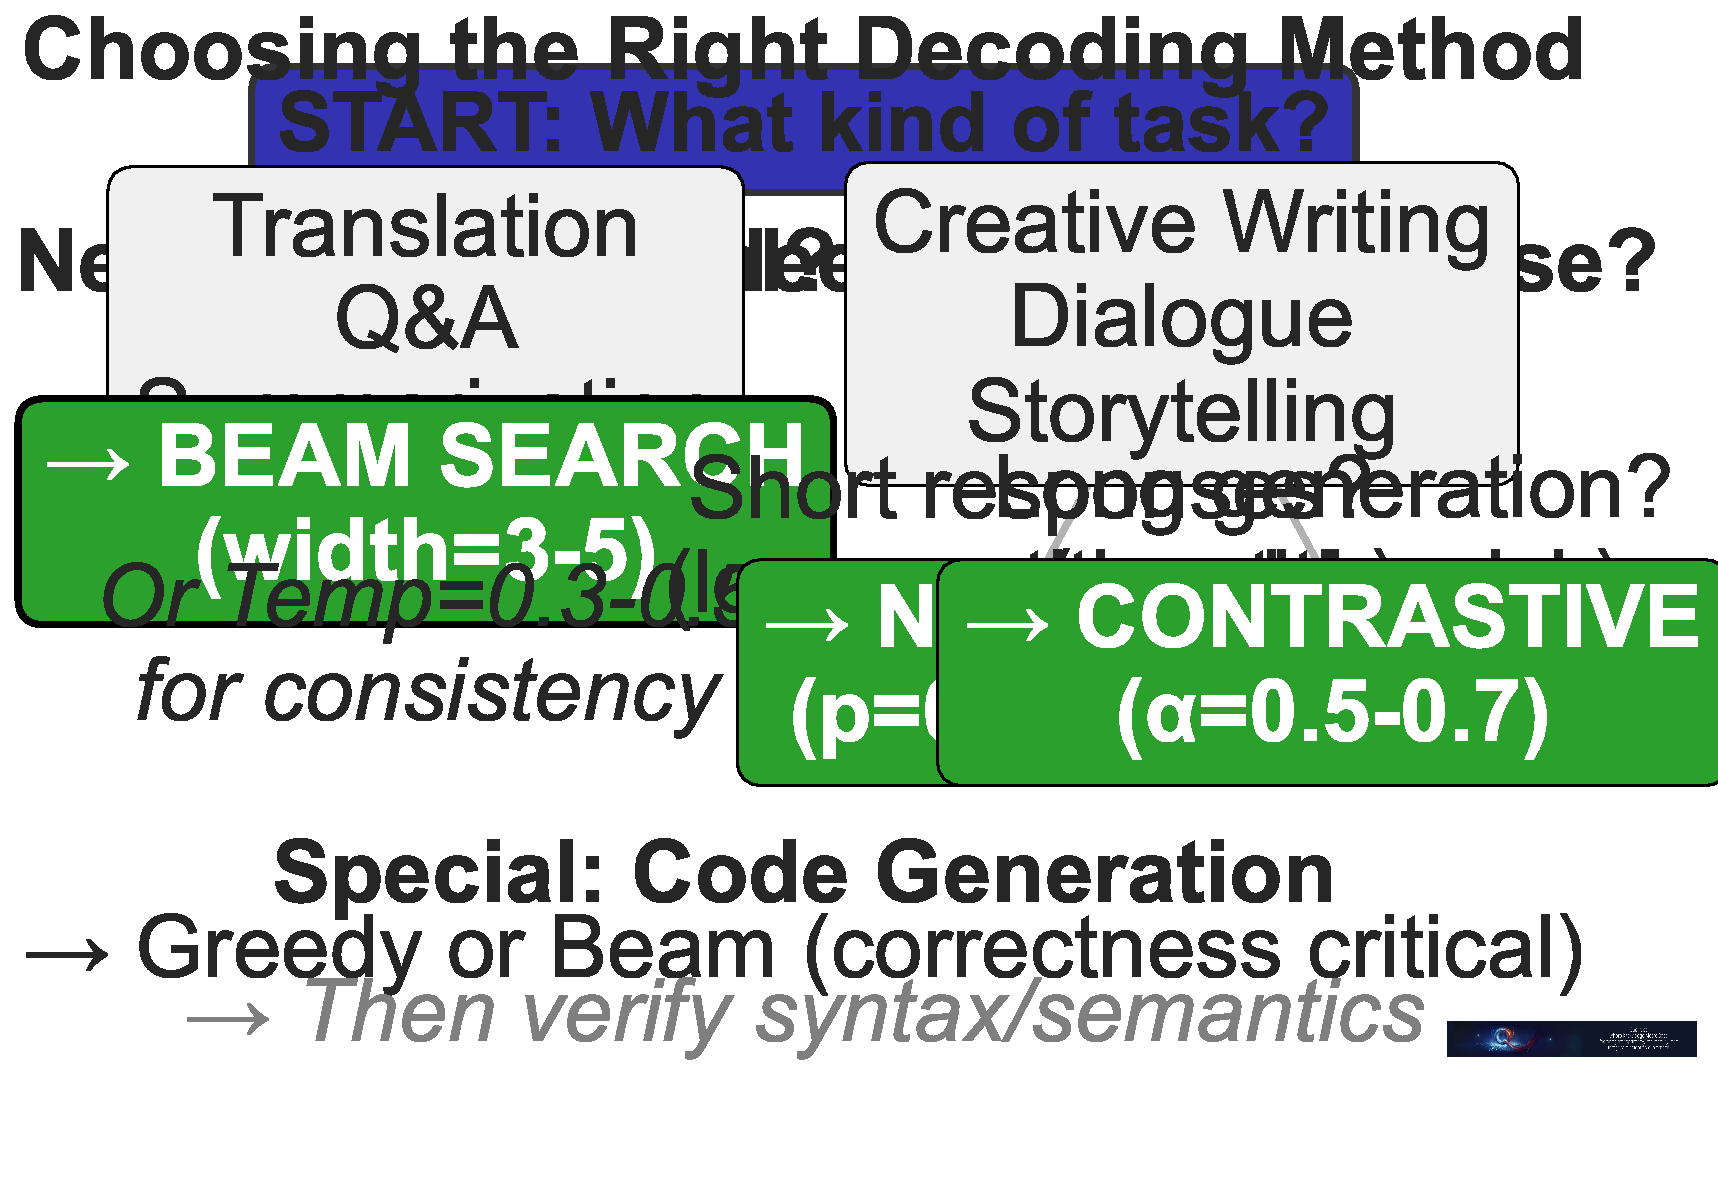
\includegraphics[width=0.70\textwidth]{../figures/task_method_decision_tree_bsc.pdf}
\end{center}
\bottomnote{Start with task requirements, follow tree to recommended method}
\end{frame}

\begin{frame}[t]{Task-Specific Recommendations (2025)}
\vspace{-0.3cm}
\begin{center}
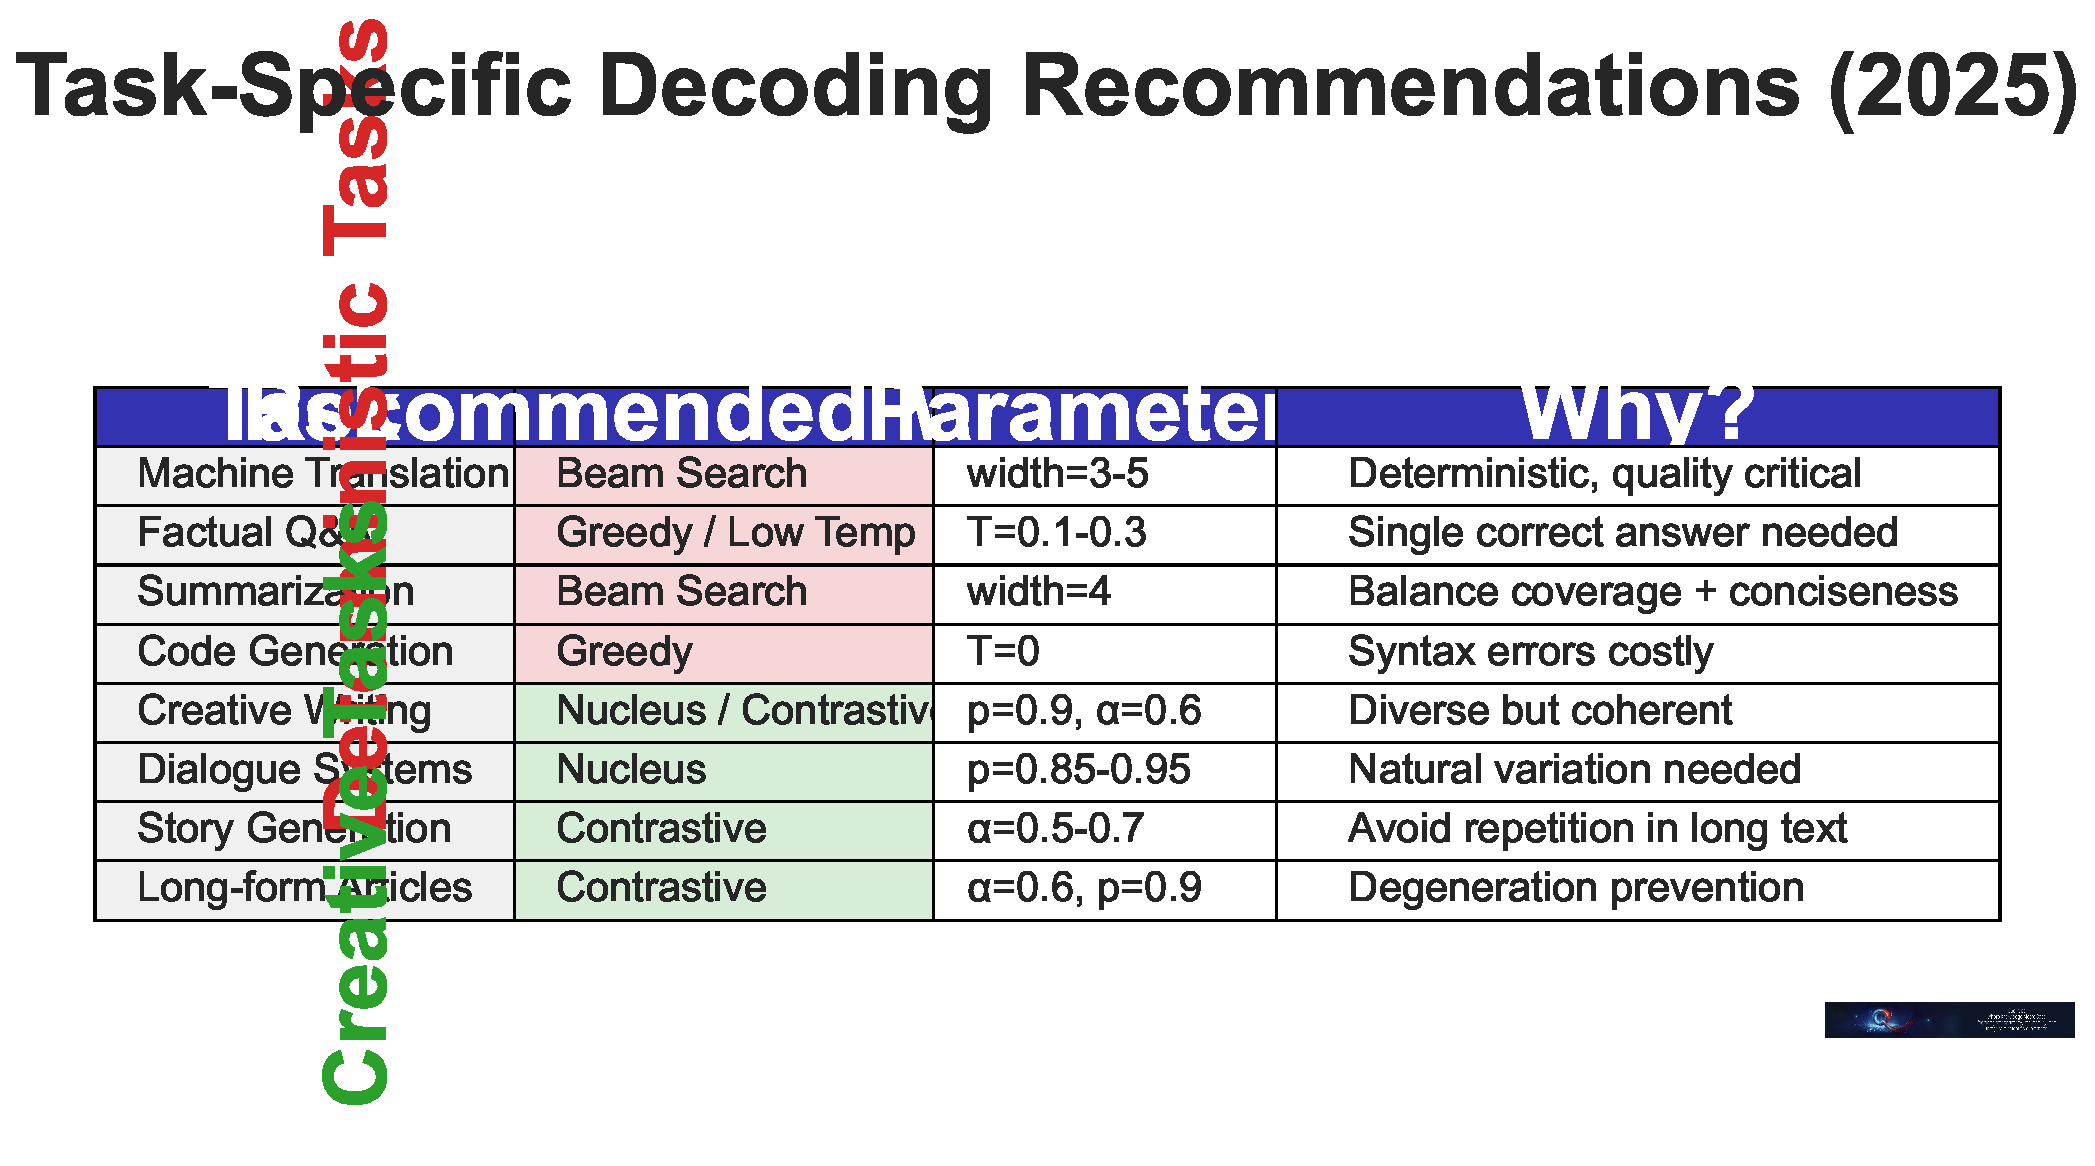
\includegraphics[width=0.75\textwidth]{../figures/task_recommendations_table_bsc.pdf}
\end{center}
\bottomnote{Comprehensive mapping from 8 common tasks to optimal decoding strategies}
\end{frame}

% Slide removed - computational_cost_comparison_bsc.pdf not generated

% === SUMMARY (4 slides: 34-37) ===
% Slide removed - decoding_comparison_bsc.pdf not generated

% Slide removed - greedy_vs_sampling_bsc.pdf not generated

% ============================================
% CHECKPOINT QUIZ 3
% ============================================

\begin{frame}[t]{Checkpoint Quiz 3: Choose the Right Method}
\textbf{Given these tasks, which method would you use?}

\begin{columns}[T]
\column{0.5\textwidth}
\begin{enumerate}
\item \textbf{Medical report summary}
   \begin{itemize}
   \item Needs: Accuracy, no hallucination
   \end{itemize}

\item \textbf{Creative story writing}
   \begin{itemize}
   \item Needs: Diversity, creativity
   \end{itemize}

\item \textbf{Code generation}
   \begin{itemize}
   \item Needs: Correctness, explore options
   \end{itemize}
\end{enumerate}

\column{0.5\textwidth}
\begin{enumerate}
\setcounter{enumi}{3}
\item \textbf{Customer service chat}
   \begin{itemize}
   \item Needs: Natural, varied responses
   \end{itemize}

\item \textbf{Legal document}
   \begin{itemize}
   \item Needs: Precise, formal
   \end{itemize}

\item \textbf{Long blog post}
   \begin{itemize}
   \item Needs: Coherent, no repetition
   \end{itemize}
\end{enumerate}
\end{columns}

\vspace{5mm}
\pause
\begin{center}
\colorbox{mlblue!20}{\parbox{0.95\textwidth}{
\centering
\textbf{Answers:}\\
1. Greedy/Low temp (T=0.1-0.3) \quad 2. Nucleus (p=0.95, T=1.0) \quad 3. Beam Search (k=3-5)\\
4. Nucleus (p=0.9, T=0.7) \quad 5. Greedy (T=0) \quad 6. Contrastive (α=0.6)
}}
\end{center}

\bottomnote{Quiz 3: Real-world task selection is crucial for quality}
\end{frame}

\begin{frame}[t]{Key Takeaways}
\begin{enumerate}
\item \textbf{6 Problems $\rightarrow$ 6 Solutions}: Each method solves specific failure mode
\item \textbf{Deterministic} (Greedy, Beam): High quality, no diversity - factual tasks
\item \textbf{Stochastic} (Temperature, Top-k, Nucleus): Diverse but variable quality
\item \textbf{Balanced} (Contrastive): Explicit degeneration prevention
\item \textbf{Task matters}: Translation $\rightarrow$ Beam | Dialogue $\rightarrow$ Nucleus | Stories $\rightarrow$ Contrastive
\item \textbf{Tradeoffs}: Speed vs Quality, Diversity vs Coherence
\end{enumerate}

\vspace{5mm}
\textbf{Modern Standard}: Nucleus (top-p=0.9) + Temperature (T=0.7) for most applications

\vspace{3mm}
\textbf{Next}: Lab - Implement all 6 methods, measure quality-diversity tradeoffs

\bottomnote{Decoding strategy matters as much as model architecture}
\end{frame}

\begin{frame}[t]{From Probabilities to Text: The Complete Journey}
\begin{center}
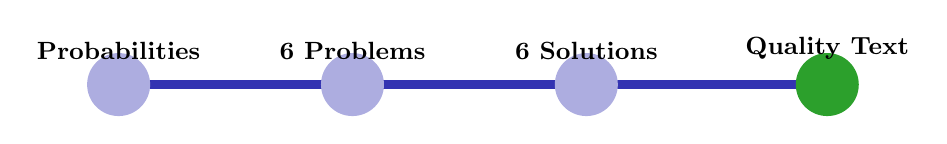
\begin{tikzpicture}[scale=0.9]
% Arrow timeline
\draw[->, line width=3pt, color=mlpurple] (0,0) -- (10,0);

% Milestones
\node[circle, fill=mllavender, minimum size=0.8cm] at (0,0) {};
\node[above=0.2cm] at (0,0) {\small\textbf{Probabilities}};

\node[circle, fill=mllavender, minimum size=0.8cm] at (3.3,0) {};
\node[above=0.2cm] at (3.3,0) {\small\textbf{6 Problems}};

\node[circle, fill=mllavender, minimum size=0.8cm] at (6.6,0) {};
\node[above=0.2cm] at (6.6,0) {\small\textbf{6 Solutions}};

\node[circle, fill=mlgreen, minimum size=0.8cm] at (10,0) {};
\node[above=0.2cm] at (10,0) {\small\textbf{Quality Text}};
\end{tikzpicture}
\end{center}

\vspace{1cm}
\textbf{What We Learned}:
\begin{itemize}
\item Models give us probability distributions (Week 3-7)
\item Converting to text has 6 fundamental challenges
\item Each decoding method addresses specific problems
\item No universal best - choose based on task requirements
\item Production systems use hybrid methods (Nucleus + Temperature)
\end{itemize}

\bottomnote{Complete pipeline from model training to text generation}
\end{frame}

% ============================================
% TECHNICAL APPENDIX (25 SLIDES: A1-A25)
% ============================================

\begin{frame}[t]
\vfill
\centering
\begin{beamercolorbox}[sep=8pt,center]{title}
\usebeamerfont{title}\Huge Technical Appendix
\end{beamercolorbox}
\vspace{0.5cm}
\large 25 slides: Complete mathematical treatment

\vspace{0.5cm}
\textcolor{mlpurple}{\textbf{A1-A5: Beam Search Mathematics}}

\textcolor{mlpurple}{\textbf{A6-A10: Sampling Mathematics}}

\textcolor{mlpurple}{\textbf{A11-A14: Contrastive Search \& Degeneration}}

\textcolor{mlpurple}{\textbf{A15-A19: Advanced Topics \& Production}}

\textcolor{mlpurple}{\textbf{A20-A25: The 6 Problems - Technical Analysis (NEW)}}
\vfill
\end{frame}

% === A1-A5: BEAM SEARCH MATHEMATICS ===

\begin{frame}[t]{A1: Beam Search Formulation}
\small
\textbf{Objective}: Find sequence $y^* = \argmax P(y | x)$

\vspace{3mm}
\textbf{Decomposition}:

$$P(y | x) = \prod_{t=1}^T P(y_t | y_{<t}, x)$$

\vspace{3mm}
\textbf{Log-probability} (more stable):

$$\log P(y | x) = \sum_{t=1}^T \log P(y_t | y_{<t}, x)$$

\vspace{3mm}
\textbf{Beam Search Approximation}:

Instead of exploring all $V^T$ sequences, maintain top-k hypotheses at each step

\vspace{3mm}
\textbf{Complexity}:

Time: $O(k \cdot V \cdot T)$ where $k$ = beam width, $V$ = vocabulary, $T$ = length

Space: $O(k \cdot T)$ to store hypotheses

\bottomnote{Beam search is tractable approximation to exact search}
\end{frame}

\begin{frame}[t]{A2: Length Normalization}
\small
\textbf{Problem}: Longer sequences have lower probabilities (more terms multiplied)

$$P(y_1, y_2, y_3, y_4) = \underbrace{0.5}_{y_1} \times \underbrace{0.5}_{y_2} \times \underbrace{0.5}_{y_3} \times \underbrace{0.5}_{y_4} = 0.0625$$

$$P(y_1, y_2) = 0.5 \times 0.5 = 0.25 > 0.0625$$

Bias toward shorter sequences!

\vspace{3mm}
\textbf{Solution}: Length normalization

$$\text{score}(y) = \frac{1}{|y|^\alpha} \log P(y)$$

where $\alpha \in [0.5, 1.0]$ (typically 0.6-0.7)

\vspace{3mm}
\textbf{Effect}:

Without: Beam search heavily biases toward short outputs

With: Fair comparison across different lengths

\bottomnote{Length normalization is essential for beam search quality}
\end{frame}

\begin{frame}[t]{A3: Beam Search Variants}
\small
\begin{columns}[T]
\column{0.48\textwidth}
\textbf{Diverse Beam Search}:

Partition beams into groups

Penalize within-group similarity

Result: More diverse hypotheses

\vspace{3mm}
\textbf{Constrained Beam Search}:

Force certain tokens to appear

Useful for: Keywords, entities

Applications: Controllable generation

\column{0.48\textwidth}
\textbf{Stochastic Beam Search}:

Sample beams instead of argmax

Combines beam + sampling

More diverse than standard beam

\vspace{3mm}
\textbf{Block n-gram Beam}:

Penalize n-gram repetition

Prevents ``the city is a city'' loops

Common in summarization

\end{columns}
\bottomnote{Many beam search variants exist for specific requirements}
\end{frame}

\begin{frame}[t]{A4: Beam Search Stopping Criteria}
\small
\textbf{When to stop expanding beams}?

\vspace{5mm}
\textbf{Method 1}: Fixed length

Stop at $T_{\max}$ tokens (simple but rigid)

\vspace{5mm}
\textbf{Method 2}: END token

Stop when beam generates special token (most common)

\vspace{5mm}
\textbf{Method 3}: Score threshold

Stop when best score cannot improve enough

$$\frac{\text{best\_incomplete}}{\text{best\_complete}} < \text{threshold}$$

\vspace{5mm}
\textbf{Method 4}: Timeout

Computational budget exceeded (production systems)

\bottomnote{Choice of stopping criterion affects output length distribution}
\end{frame}

\begin{frame}[t]{A5: Beam Search Limitations}
\small
\textbf{Fundamental Issues}:

\begin{enumerate}
\item \textbf{Exposure bias}: Trained with teacher forcing, tested with own outputs
\item \textbf{Label bias}: Cannot compare sequences of different prefixes fairly
\item \textbf{Repetition}: Still can loop (``the city is a major city'')
\item \textbf{Bland outputs}: Maximizes probability, not interestingness
\item \textbf{Search errors}: May miss better sequences outside beam
\end{enumerate}

\vspace{5mm}
\textbf{When Beam Search Fails}:

Open-ended generation (dialogue, stories)

Long-form text (repetition accumulates)

Creative tasks (probability $\neq$ quality)

\vspace{5mm}
$\rightarrow$ Need sampling-based methods

\bottomnote{Beam search optimizes wrong objective for creative tasks}
\end{frame}

% === A6-A10: SAMPLING MATHEMATICS ===

\begin{frame}[t]{A6: Sampling as Inference}
\small
\textbf{Goal}: Sample $y \sim P(y | x)$ instead of $\argmax P(y | x)$

\vspace{3mm}
\textbf{Ancestral Sampling}:

For $t = 1$ to $T$:

\hspace{1cm} Compute $P(y_t | y_{<t}, x)$

\hspace{1cm} Sample $y_t \sim P(\cdot | y_{<t}, x)$

\vspace{3mm}
\textbf{Properties}:

Stochastic: Different output each time

Explores full distribution (in expectation)

Can generate low-probability sequences

\vspace{3mm}
\textbf{Variants}:

Temperature: Reshape distribution before sampling

Top-k: Truncate distribution before sampling

Nucleus: Dynamic truncation before sampling

\bottomnote{Sampling enables diversity but loses quality guarantees}
\end{frame}

\begin{frame}[t]{A7: Temperature Mathematics}
\small
\textbf{Softmax with Temperature}:

$$p_i(T) = \frac{\exp(z_i / T)}{\sum_{j=1}^V \exp(z_j / T)}$$

\vspace{3mm}
\textbf{Limiting Cases}:

$T \rightarrow 0$: $p_i \rightarrow \begin{cases} 1 & \text{if } i = \argmax z \\ 0 & \text{otherwise} \end{cases}$ (greedy)

$T \rightarrow \infty$: $p_i \rightarrow 1/V$ (uniform)

\vspace{3mm}
\textbf{Entropy Analysis}:

Entropy $H(p) = -\sum p_i \log p_i$ measures randomness

$H$ increases monotonically with $T$

Low $T$ ($<$0.5): $H \approx 0$ (deterministic)

High $T$ ($>$2.0): $H \approx \log V$ (maximum entropy)

\bottomnote{Temperature provides continuous control over distribution entropy}
\end{frame}

\begin{frame}[t]{A8: Top-k Mathematics}
\small
\textbf{Formal Definition}:

Let $\sigma$ = permutation sorting probabilities descending

$$V_k = \{w_{\sigma(1)}, w_{\sigma(2)}, ..., w_{\sigma(k)}\}$$

Truncated distribution:

$$p'(w) = \begin{cases} \frac{p(w)}{\sum_{w' \in V_k} p(w')} & \text{if } w \in V_k \\ 0 & \text{otherwise} \end{cases}$$

\vspace{3mm}
\textbf{Information Loss}:

Original entropy: $H(p) = -\sum_{i=1}^V p_i \log p_i$

After top-k: $H(p') = -\sum_{i=1}^k p'_i \log p'_i < H(p)$

Loss $\approx \sum_{i=k+1}^V p_i \log(1/p_i)$ (tail information)

\bottomnote{Top-k sacrifices tail probability mass for sampling quality}
\end{frame}

\begin{frame}[t]{A9: Nucleus (Top-p) Mathematics}
\small
\textbf{Formal Definition}:

$$V_p = \min \left\{ V' \subseteq V : \sum_{w \in V'} p(w) \geq p \right\}$$

Smallest set with cumulative mass $\geq p$

\vspace{3mm}
\textbf{Dynamic Vocabulary Size}:

$$|V_p| = \min \{k : \sum_{i=1}^k p_{\sigma(i)} \geq p\}$$

Adapts to distribution shape:

Peaked: Small $|V_p|$ (2-5 tokens)

Flat: Large $|V_p|$ (50+ tokens)

\vspace{3mm}
\textbf{Why Nucleus $>$ Top-k}:

Top-k: Fixed $k$ regardless of $p(w)$ distribution

Nucleus: Adapts $k$ to achieve consistent probability mass

\bottomnote{Nucleus automatically adjusts vocabulary to distribution characteristics}
\end{frame}

\begin{frame}[t]{A10: Sampling Quality Metrics}
\small
\begin{columns}[T]
\column{0.48\textwidth}
\textbf{Quality Metrics}:

\textbf{Perplexity}: $\exp(-\frac{1}{T} \sum \log p(y_t))$

Lower = better

\vspace{3mm}
\textbf{BLEU} (translation):

N-gram overlap with reference

0-100 scale

\vspace{3mm}
\textbf{Human evaluation}:

Fluency (1-5)

Relevance (1-5)

\column{0.48\textwidth}
\textbf{Diversity Metrics}:

\textbf{Distinct-n}: $\frac{\text{unique n-grams}}{\text{total n-grams}}$

Higher = more diverse

\vspace{3mm}
\textbf{Self-BLEU}:

BLEU of output vs other outputs

Lower = more diverse

\vspace{3mm}
\textbf{Repetition Rate}:

$\frac{\text{repeated n-grams}}{\text{total n-grams}}$

Lower = less repetitive

\end{columns}
\bottomnote{Need both quality AND diversity metrics to evaluate decoding}
\end{frame}

% === A11-A14: CONTRASTIVE SEARCH & DEGENERATION ===

\begin{frame}[t]{A11: The Degeneration Problem (Formal)}
\small
\textbf{Definition}: Model-generated text with unnatural repetitions

\vspace{3mm}
\textbf{Why It Happens}:

\begin{enumerate}
\item Model trained on natural text (low repetition)
\item But generation maximizes $P(y_t | y_{<t})$
\item Recent context $y_{<t}$ influences $P$
\item Creates positive feedback: high prob word $\rightarrow$ context $\rightarrow$ same high prob word
\end{enumerate}

\vspace{3mm}
\textbf{Quantifying Degeneration}:

Repetition rate in greedy: 15-30\% (depending on domain)

Repetition rate in human text: 2-5\%

Gap = degeneration problem

\vspace{3mm}
\textbf{Examples}:

``\textit{The city is a major city in the United States. The city...}''

``\textit{I think that I think that I think...}''

\bottomnote{Maximizing probability does not equal natural text}
\end{frame}

\begin{frame}[t]{A12: Contrastive Search Objective}
\small
\textbf{Scoring Function}:

$$\text{score}(w_t) = (1 - \alpha) \times \underbrace{P(w_t | y_{<t})}_{\text{model confidence}} - \alpha \times \underbrace{\max_{w_i \in y_{<t}} \text{sim}(w_t, w_i)}_{\text{context similarity}}$$

where $\alpha \in [0, 1]$ controls tradeoff

\vspace{3mm}
\textbf{Similarity Function}:

$$\text{sim}(w_i, w_j) = \frac{h_i \cdot h_j}{||h_i|| \cdot ||h_j||}$$ (cosine similarity)

using token embeddings $h$

\vspace{3mm}
\textbf{Algorithm}:

\begin{enumerate}
\item Get top-k candidates by probability
\item For each candidate, compute similarity to all tokens in $y_{<t}$
\item Apply penalty: score = prob - $\alpha \times$ max\_similarity
\item Select candidate with highest score
\end{enumerate}

\bottomnote{Contrastive search explicitly penalizes copying recent context}
\end{frame}

\begin{frame}[t]{A13: Contrastive Search Parameters}
\small
\begin{columns}[T]
\column{0.48\textwidth}
\textbf{Alpha} ($\alpha$):

$\alpha = 0$: Pure greedy (no penalty)

$\alpha = 0.6$: Balanced (recommended)

$\alpha = 1.0$: Maximum diversity (risky)

\vspace{3mm}
\textbf{Typical Settings}:

Short text ($<$100 tokens): $\alpha = 0.4-0.5$

Medium ($<$500): $\alpha = 0.5-0.6$

Long (500+): $\alpha = 0.6-0.7$

\column{0.48\textwidth}
\textbf{Top-k for Candidates}:

$k = 4$: Fast, focused

$k = 6$: Balanced (default)

$k = 10$: Diverse

\vspace{3mm}
\textbf{Computational Cost}:

For each step:
\begin{itemize}
\item Compute similarities: $O(k \times t)$
\item $t$ grows with generation
\end{itemize}

Total: $O(k \times T^2)$

12$\times$ slower than greedy

\end{columns}
\bottomnote{Hugging Face default: $\alpha$=0.6, k=4}
\end{frame}

\begin{frame}[t]{A14: Degeneration Analysis}
\small
\textbf{Research Findings} (2024-2025):

\begin{itemize}
\item Greedy decoding repetition: 18-25\% (GPT-2), 12-18\% (GPT-3)
\item Nucleus sampling repetition: 8-12\% (still above human 3-5\%)
\item Contrastive search repetition: 4-7\% (closest to human)
\end{itemize}

\vspace{3mm}
\textbf{Why Probability Maximization Fails}:

Training objective: Next token prediction

But generation requires: Global coherence

Mismatch: Local optimum $\neq$ global quality

\vspace{3mm}
\textbf{Solutions Hierarchy}:

\begin{enumerate}
\item Temperature/Top-k/Nucleus: Reduce greedy's determinism
\item Contrastive: Explicit degeneration penalty
\item RLHF/DPO: Align model with human preferences (different lecture)
\end{enumerate}

\bottomnote{Contrastive search addresses fundamental limitation of likelihood-based decoding}
\end{frame}

% === A15-A19: ADVANCED TOPICS ===

\begin{frame}[t]{A15: Hybrid Decoding Methods}
\small
\textbf{Combining Strategies}:

\vspace{3mm}
\textbf{Nucleus + Temperature}:

Apply temperature THEN nucleus

$$p_i(T) = \softmax(z / T), \quad \text{then} \quad V_p \gets \text{nucleus}(p_i(T))$$

Used by GPT-3 API, ChatGPT

\vspace{3mm}
\textbf{Beam + Sampling}:

Beam search with stochastic selection

Keep top-k, sample from them (not argmax)

\vspace{3mm}
\textbf{Contrastive + Nucleus}:

Nucleus for candidate generation

Contrastive scoring for selection

Best of both worlds

\bottomnote{Hybrid methods leverage complementary strengths}
\end{frame}

\begin{frame}[t]{A16: Constrained Decoding (2025)}
\small
\textbf{Goal}: Force certain tokens/patterns to appear

\vspace{3mm}
\textbf{Lexically Constrained}:

Must include keywords: \{``AI'', ``ethics'', ``safety''\}

Beam search variant: Track constraint satisfaction

\vspace{3mm}
\textbf{Format Constraints}:

JSON output: Force structure \{``key'': ``value''\}

Code: Force syntactic validity

\vspace{3mm}
\textbf{NeuroLogic Decoding} (2021):

Beam search + constraint satisfaction

Optimal for: Keyword-based generation

\vspace{3mm}
\textbf{Production Use Cases}:

Structured data extraction (force JSON)

Controllable summarization (force keywords)

Code generation (force syntax)

\bottomnote{Constrained decoding enables controllable generation}
\end{frame}

\begin{frame}[t]{A17: Computational Complexity Comparison}
\small
\begin{center}
\begin{tabular}{lccc}
\hline
\textbf{Method} & \textbf{Time per token} & \textbf{Total complexity} & \textbf{Relative speed} \\
\hline
Greedy & $O(V)$ & $O(V \times T)$ & 1.0$\times$ (baseline) \\
Temperature & $O(V)$ & $O(V \times T)$ & 1.1$\times$ (softmax overhead) \\
Top-k & $O(V)$ & $O(V \times T)$ & 1.2$\times$ (sorting) \\
Nucleus & $O(V \log V)$ & $O(V \log V \times T)$ & 1.3$\times$ (sort + cumsum) \\
Beam (k=5) & $O(k \times V)$ & $O(k \times V \times T)$ & 4.5$\times$ (k=5) \\
Contrastive & $O(k \times T)$ & $O(k \times T^2)$ & 12$\times$ (similarity) \\
\hline
\end{tabular}
\end{center}

\vspace{3mm}
\textbf{Key Insight}: Contrastive's $T^2$ term makes it expensive for long sequences

\vspace{3mm}
\textbf{Practical Impact} (1000-token generation):

Greedy: 2.5 seconds

Nucleus: 3.2 seconds (best choice)

Beam: 11 seconds

Contrastive: 30 seconds (only if quality critical)

\bottomnote{Computational cost matters for production deployment}
\end{frame}

% Slide removed - production_settings_bsc.pdf not generated

\begin{frame}[t]{A19: Future Directions \& Open Problems}
\small
\textbf{Active Research Areas} (2025):

\begin{enumerate}
\item \textbf{Quality-diversity optimization}: Multi-objective search methods
\item \textbf{Learned decoding}: Train models to decode better (RLHF, DPO)
\item \textbf{Speculative decoding}: Parallel generation for speed (4-8$\times$ faster)
\item \textbf{Adaptive methods}: Choose strategy dynamically during generation
\item \textbf{Energy-based decoding}: Score sequences globally (not token-by-token)
\end{enumerate}

\vspace{5mm}
\textbf{Open Problems}:

How to automatically select best $T$, $p$, $k$, $\alpha$ for new task?

How to balance fluency + factuality + creativity simultaneously?

How to decode efficiently for 100K+ token outputs?

\vspace{5mm}
\textbf{Trend}: Moving from hand-tuned parameters to learned decoding strategies

\bottomnote{Decoding is an active research area with many open questions}
\end{frame}

% === A20-A25: THE 6 PROBLEMS - TECHNICAL ANALYSIS (NEW) ===

\begin{frame}[t]
\vfill
\centering
\begin{beamercolorbox}[sep=8pt,center]{title}
\usebeamerfont{title}\Large Appendix B: The 6 Problems
\end{beamercolorbox}
\vspace{0.5cm}
Technical Analysis of Each Failure Mode

\vspace{0.5cm}
Next 6 slides: Detailed technical analysis pairing:

\textbf{Top}: Technical level explanation

\textbf{Bottom}: Concrete output failure
\vfill
\end{frame}

\begin{frame}[t]{B1: Problem 1 Technical Analysis}
\textbf{Technical Issue} (Level):
\vspace{-0.2cm}
\begin{center}
\includegraphics[width=0.85\textwidth]{../figures/framing3_level1_too_deterministic.pdf}
\end{center}

\vspace{2mm}
\textbf{Concrete Failure} (Output):
\vspace{-0.2cm}
\begin{center}
\includegraphics[width=0.85\textwidth]{../figures/problem1_repetition_output_bsc.pdf}
\end{center}
\end{frame}

\begin{frame}[t]{B2: Problem 2 Technical Analysis}
\textbf{Technical Issue} (Level):
\vspace{-0.2cm}
\begin{center}
\includegraphics[width=0.85\textwidth]{../figures/framing3_level2_too_random.pdf}
\end{center}

\vspace{2mm}
\textbf{Concrete Failure} (Output):
\vspace{-0.2cm}
\begin{center}
\includegraphics[width=0.85\textwidth]{../figures/problem2_diversity_output_bsc.pdf}
\end{center}
\end{frame}

\begin{frame}[t]{B3: Problem 3 Technical Analysis}
\textbf{Technical Issue} (Level):
\vspace{-0.2cm}
\begin{center}
\includegraphics[width=0.85\textwidth]{../figures/framing3_level3_inflexible_filter.pdf}
\end{center}

\vspace{2mm}
\textbf{Concrete Failure} (Output):
\vspace{-0.2cm}
\begin{center}
\includegraphics[width=0.85\textwidth]{../figures/problem3_balance_output_bsc.pdf}
\end{center}
\end{frame}

\begin{frame}[t]{B4: Problem 4 Technical Analysis}
\textbf{Technical Issue} (Level):
\vspace{-0.2cm}
\begin{center}
\includegraphics[width=0.85\textwidth]{../figures/framing3_level4_missing_paths.pdf}
\end{center}

\vspace{2mm}
\textbf{Concrete Failure} (Output):
\vspace{-0.2cm}
\begin{center}
\includegraphics[width=0.85\textwidth]{../figures/problem4_paths_output_bsc.pdf}
\end{center}
\end{frame}

\begin{frame}[t]{B5: Problem 5 Technical Analysis}
\textbf{Technical Issue} (Level):
\vspace{-0.2cm}
\begin{center}
\includegraphics[width=0.85\textwidth]{../figures/framing3_level5_still_repetitive.pdf}
\end{center}

\vspace{2mm}
\textbf{Concrete Failure} (Output):
\vspace{-0.2cm}
\begin{center}
\includegraphics[width=0.85\textwidth]{../figures/problem5_distribution_output_bsc.pdf}
\end{center}
\end{frame}

\begin{frame}[t]{B6: Problem 6 Technical Analysis}
\textbf{Technical Issue} (Level):
\vspace{-0.2cm}
\begin{center}
\includegraphics[width=0.85\textwidth]{../figures/framing3_level6_need_balance.pdf}
\end{center}

\vspace{2mm}
\textbf{Concrete Failure} (Output):
\vspace{-0.2cm}
\begin{center}
\includegraphics[width=0.85\textwidth]{../figures/problem6_speed_output_bsc.pdf}
\end{center}
\end{frame}

\end{document}
